%*****************************************
\chapter{Geospatial environmental and techno-economic framework for	sustainable phosphorus management at livestock facilities}\label{ch:Tool}
\chaptermark{Environmental and techno-economic framework for P management}
%*****************************************
\section*{Abstract}
Nutrient pollution of waterbodies is a major worldwide water quality problem. Excessive use and discharge of nutrients can lead to eutrophication and algal blooms in fresh and marine waters, resulting in environmental problems associated with hypoxia, public health issues related to the release of toxins and freshwater scarcity. A promising option to address this problem is the recovery of nutrient releases prior to being discharged into the environment. Driven by the sustainable materials management concept, the COW2NUTRIENT (Cattle Organic Waste to NUTRIent and ENergy Technologies) framework is developed for the techno-economic evaluation and selection of nutrient recovery systems at livestock facilities. Environmental vulnerability to nutrient pollution determined through a geographic information system (GIS)-based model and techno-economic information of different state-of-the-art nutrient management technologies are combined in a multi-criteria decision analysis (MCDA) model, resulting in the selection and economic analysis of the most suitable process for each studied livestock facility. This framework has been employed for studying the implementation of sustainable phosphorus management systems at 2,217 livestock facilities in the Great Lakes area, resulting in capital expenses of 2.5 billion USD if only phosphorus recovery technologies are installed, and up to 5.2 billion USD if nutrient management is combined with biogas and power production. However, considering potential economic incentives for the recovery of phosphorus, net revenues up to 230 million USD per year can be achieved. Therefore, the framework presented reveals the potential of implementing nutrient management systems at regional scale for the abatement of phosphorus releases from livestock facilities.

\bigskip
\textbf{Keywords:} Organic waste; Harmful algal blooms; Nutrient pollution; Livestock waste; Phosphorus recovery

\newpage

\section*{Resumen}
La contaminación por nutrientes de las masas de agua es uno de los principales problemas de calidad del agua en todo el mundo. El uso y el vertido excesivos de nutrientes pueden provocar la eutrofización y la proliferación de algas en las aguas dulces y marinas, lo que da lugar a problemas medioambientales relacionados con la hipoxia, cuestiones de salud pública relacionadas con la liberación de toxinas y escasez de agua dulce. Una opción prometedora para abordar este problema es la recuperación de los vertidos de nutrientes antes de ser vertidos al medio ambiente. Impulsado por el concepto de gestión sostenible de materiales, se ha desarrollado el marco COW2NUTRIENT (Cattle Organic Waste to NUTRIent and ENergy Technologies) para la evaluación y selección tecnoeconómica de sistemas de recuperación de nutrientes en instalaciones ganaderas. La vulnerabilidad ambiental a la contaminación por nutrientes, determinada a través de un modelo basado en un sistema de información geográfica (SIG), y la información tecno-económica de diferentes tecnologías de gestión de nutrientes de última generación se combinan en un modelo de análisis de decisiones multicriterio (MCDA), dando como resultado la selección y el análisis económico del proceso más adecuado para cada instalación ganadera estudiada. Este marco se ha empleado para estudiar la implantación de sistemas de gestión sostenible del fósforo en 2.217 instalaciones ganaderas de la zona de los Grandes Lagos, lo que supone unos gastos de capital de 2.500 millones de dólares si sólo se instalan tecnologías de recuperación de fósforo, y de hasta 5.200 millones de dólares si la gestión de nutrientes se combina con la producción de biogás y energía. Sin embargo, si se tienen en cuenta los posibles incentivos económicos para la recuperación de fósforo, se pueden conseguir ingresos netos de hasta 230 millones de dólares al año. Por lo tanto, el marco presentado revela el potencial de la aplicación de sistemas de gestión de nutrientes a escala regional para la reducción de las emisiones de fósforo de las instalaciones ganaderas.

\bigskip
\textbf{Palabras clave:} Residuos orgánicos; Florecimiento de algas; Contaminación por nutrientes; Residuos ganaderos; Recuperación de fósforo

\newpage

\begin{refsection}[referencesCh4]
\section{Introduction}
Phosphorus is a source of concern for modern societies. On the one hand, nutrient pollution of waterbodies is one of the major water quality problems worldwide, resulting in environmental issues as a consequence of the eutrophication of waterbodies, and the occurrence of cyanobacteria and harmful algal blooms (HABs). Surveys reveal that eutrophication is a global problem, reporting that 54\% of lakes in Asia, 53\% in Europe, 48\% in North America, 41\% in South America, and 28\% in Africa are eutrophic \citep{ansari_eutrophication_2010}. In addition to eutrophication, hypoxia of aquatic ecosystems is associated with the aerobic degradation of the algal biomass by bacteria, shifting the distribution of aquatic species and releasing toxins in drinking water sources \citep{sampat_economic_2018}. Although eutrophication is affected by several factors, such as temperature and the self-purification capacity of waterbodies, the primary limiting factor for eutrophication is often the phosphate concentration \citep{Ullmanns}. Aside from disturbing aquatic ecosystems, eutrophication also contributes to climate change, emitting large amounts of strong greenhouse gases as a consequence of the biomass degradation, such as CH\textsubscript{4} and N\textsubscript{2}O \citep{beaulieu_eutrophication_2019}. On the other hand, phosphorus is an essential nutrient for living organisms, and a key element for maintaining agricultural productivity. However, phosphorus is a resource very sensitive to depletion, since extractable deposits of phosphorus rock are limited and there is no known substitute or synthetic replacement. Projections estimate limited availability of phosphate over the next century \citep{cordell_story_2009}. Therefore, in addition to the environmental perspective, the search for phosphorus recycling processes is a major driving force for the development of nutrient recovery systems \citep{reijnders2014phosphorus}.

Agricultural activities are one of the main contributors to human-based phosphorus releases \citep{Dzombak}, including non-point source releases by over-use of fertilizers in croplands, point source releases originated from the disposal of livestock waste, and nutrient legacy that have accumulated in watersheds due to historical phosphorus releases. Focusing on the point source releases generated by the cattle industry, these result from the production of large amounts of livestock organic waste, containing substantial amounts of phosphate and ammonia. \citet{Sampat2017} presented the link between the presence of livestock facilities and higher concentrations of phosphorus in soil, resulting in increased nutrient runoff to waterbodies. While for animals on pasture, organic waste should not be a source of concern if stocking rates are not excessive, for concentrated animal feeding operations (CAFOs) manure should be properly managed due to the high rates and spatial concentration of the organic waste generated.
A common practice to recycle the nutrients contained in the organic waste is the land application of the manure. However, since the high-water content of manure makes its transportation to nutrient deficient locations difficult and expensive, it is usually spread in the surroundings of the CAFOs, leading to surplus of nutrients in soils and phosphorus runoff to waterbodies \citep{USDAHandbook}.

The implementation of nutrient recovery technologies at livestock facilities to recover phosphorus from cattle manure is a promising approach to recycle and leverage nutrients more efficiently, mitigating the nutrient pollution of waterbodies \citep{li2021toward}. However, the technologies that can be implemented at CAFOs differ widely in aspects such as phosphorus recovery performance, final products obtained, capital expenses, and operational costs. Additionally, different levels of environmental vulnerability to eutrophication may require the use of different P recovery processes, searching for the most effective balance between P recovery efficiency and cost.
Previous efforts for the technical evaluation of different phosphorus recovery technology have been performed, resulting in processes with proven technical feasibility for phosphorus recovery. Particularly, there exists a considerable body of literature on the production of struvite \citep{muhmood2019formation}. Other mature processes for the recovery of phosphorus are the formation of calcium precipitates \citep{berg2006phosphorus}, and systems based on physical separations \citep{church_novel_2016}. Additionally, novel processes are currently under development, such as membrane separation processes \citep{li2020application}, microalgae-based processes \citep{robles2020new}, adsorption using biochar \citep{wang2020phosphorus}, and electrochemical processes \citep{belarbi2020bench}.
Moreover, a decision-making framework has been developed for the selection and implementation of phosphorus recovery systems in urban areas \citep{pearce2015phosphorus}.
However, to the best of the authors knowledge, there are no specific frameworks to study the implementation of phosphorus recovery systems at livestock facilities considering GIS environmental and techno-economic dimensions.

In this work, we propose a novel framework, COW2NUTRIENT (Cattle Organic Waste to NUTRIent and ENergy Technologies), for the assessment and selection of phosphorus recovery technologies at CAFOs based on environmental and techno-economic criteria. This framework combines eutrophication risk data at subbasin level and the techno-economic assessment of six state-of-the-art phosphorus recovery processes in a multi-criteria decision analysis (MCDA) model. This information is normalized and aggregated for the selection of the most suitable technology for each analyzed CAFO. The goal is to develop a flexible framework able to balance the operating cost of the systems and P recovery efficiency as a function of the environmental vulnerability to eutrophication of each region. The minimization of operating costs is prioritized in regions with low eutrophication risk, while the efficiency of P recovery is the most relevant criteria in regions affected by nutrient pollution. Also, COW2NUTRIENT aims to provide a useful framework for designing and evaluating effective GIS-based incentives and regulatory policies to control and mitigate nutrient pollution of waterbodies. The practicability of the proposed framework is assessed by studying and designing the implementation of P recovery systems at 2,217 current livestock facilities in the Great Lakes area.

\section{Methods}
COW2NUTRIENT framework is comprised by three models, i.e. environmental geographic information, techno-economic, and multi-criteria decision analysis models, in order to integrate the geographic data on vulnerability to nutrient pollution, and the technical and economic information of the nutrient recovery systems through an MCDA model, as shown in Figure \ref{fig:tool_diagram}. First, the geographic location of the individual facilities (longitude and latitude) is supplied to the environmental GIS model to determine the vulnerability level to nutrient pollution of the region where the studied CAFOs are located. Secondly, data regarding the number and type of animals at the facility (i.e., beef and dairy cattle, adult animals, heifers, and calves) are entered into the techno-economic model to capture the characteristics of the livestock facility evaluated. Data reported by the US Department of Agriculture were considered for manure generation ratios \citep{Kellog2010} and composition \citep{USDAHandbook}. These values are collected in Table 3S of the Supplementary Material. In addition, economic data are fed into the techno-economic model for economic performance evaluation purposes, including the value of incentives received for phosphorus recovery (in the form of P credits), and for the generation of bio-based methane or electricity (in form of Renewable Energy Certificate (REC) and Renewable Identification Number (RIN) respectively). The output data from the techno-economic and environmental geographic information models are imported in the MCDA model. In this module, the data is normalized and aggregated, returning a composite index for each technology. This composite index is used to score and rank the nutrient recovery systems based on their performance. All models have been developed using Python \citep{Python}.


\begin{figure}[h]
	\centering
	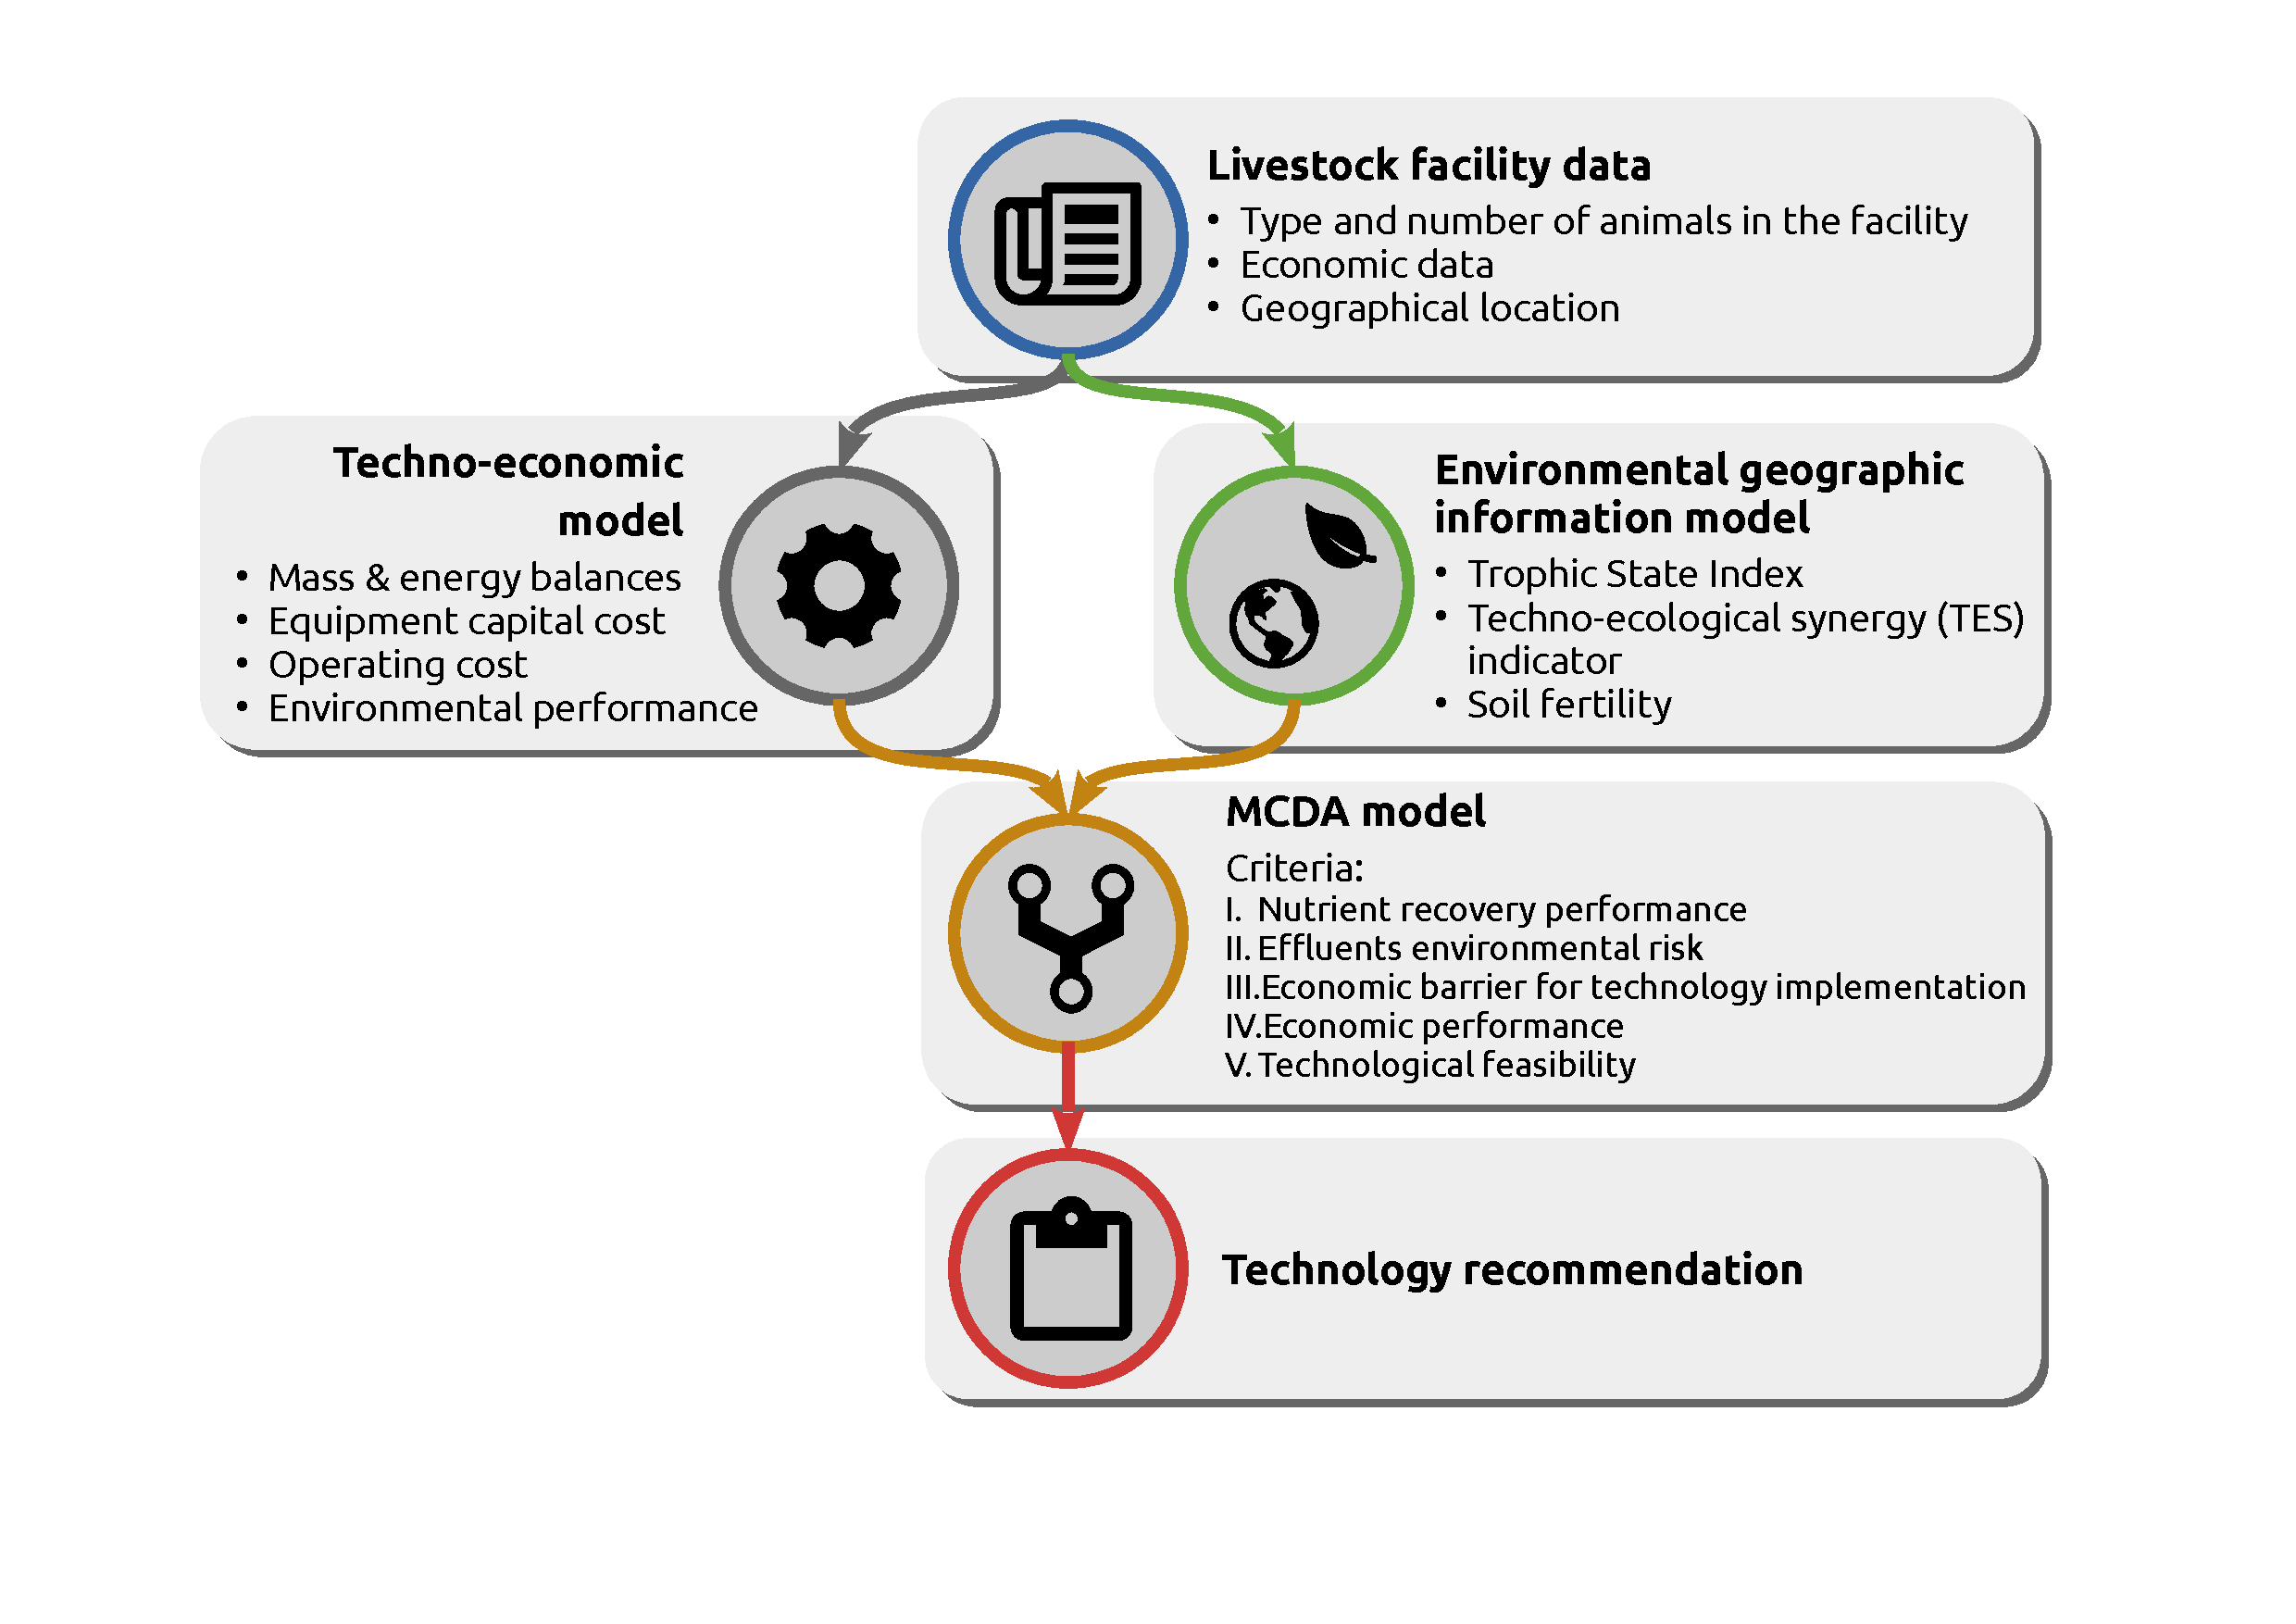
\includegraphics[width=0.95\linewidth, trim={3cm 4cm 4cm 1.5cm},clip]{gfx/Chapter4/tool_diagram_v4color.pdf} 
	\caption{Structure of the COW2NUTRIENT decision support framework for the assessment and selection of phosphorus recovery systems.}
	\label{fig:tool_diagram}
\end{figure}

\subsection{Environmental geographic information model}
The environmental vulnerability to nutrient pollution of the area where the livestock facilities are located determines the preference (i.e., ranks the importance) of each criterion. 
Three indicators are used to evaluate the eutrophication risk of each region studied at subbasin spatial resolution. The trophic state of waterbodies is evaluated through the Trophic State Index \citep{carlson_trophic_1977}, determining their eutrophication level. The phosphorus saturation of soils, which can result in the transport of phosphorus to waterbodies by run-off, is evaluated through Mehlich 3 phosphorus concentration \citep{Espinoza2006}. Finally, the balance between phosphorus releases and uptakes from  anthropogenic activities is assessed through the techno-ecological synergy metric \citep{TESmetric}, determining if there is a net accumulation or depletion of phosphorus in a region over time. The use of these three indicators makes it possible to determine if there exist an immediate risk of eutrophication in the region studied (eutrophized waterbodies), a long-term risk (moderate value of TSI, soils saturated by phosphorus, or phosphorus releases and uptakes from  anthropogenic activities unbalanced), or if there is no risk of eutrophication (phosphorus uptakes and releases are balanced). Detailed descriptions of the performed data analysis, and maps for the contiguous US are provided in Section 1 of the Supplementary Material.

\subsubsection{Spatial resolution}
A watershed is defined as the region draining all the streams and rainfall to a common waterbody, defining the geographic limits for the collection of runoff elements. US watersheds are designated by the US Geological Survey through the Hydrologic Unit Code (HUC) system. The HUC system divides the US into regions, subregions, basins, subbasins, watersheds, and subwatersheds. Each hydrologic unit of these six levels is identified hierarchically by a unique numeric code from 2 to 12 digits (i.e., HUC2 to HUC12).
The spatial resolution of this study is the contiguous United States at the subbasin level, defined by the HUC system at 8 digits (HUC8) \citep{HUC8}.

\subsubsection{Trophic State Index}
The Trophic State Index (TSI) is a metric proposed by \citet{carlson_trophic_1977} to determine the trophic status of waterbodies \citep{QAPP2012}. The TSI of a waterbody is scored in a range from 0 to 100 representing its throphic state, as shown in Table \ref{table:TSI_relation}. Oligotrophic and mesotrophic states denote low and intermediate biomass productivities, while eutrophic and hypereutrophic states are referred to waterbodies with high biological productivity and frequent algal blooms. Combined data for chl-$\alpha$ and total phosphorus concentrations retrieved from the National Lakes Assessments conducted by the US EPA in 2007 and 2012 \citep{NLA2012, NLA2007} is used to determine the Trophic State Index of lentic waters in the contiguous US. No TSI values were assigned to the watersheds without reported data. Correlations to estimate the TSI from chlorophyll-$\alpha$ and total phosphorus concentrations are collected in Section 1 of Supplementary Material.

\begin{table}[h]
	\centering
	\caption{Relation between TSI value and trophic class.}
	\label{table:TSI_relation}
	\resizebox{0.9\columnwidth}{!}{
	\begin{tabular}{@{}lllll@{}}
		\toprule
		{TSI}           & \textless 40 & 40-50       & 50-70     & \textgreater{}70 \\ \midrule
		{Trophic Class} & Oligotrophic & Mesotrophic & Eutrophic & Hypereutrophic   \\ \bottomrule
	\end{tabular}
	}
\end{table}

\subsubsection{Techno-ecological synergy sustainability metric}
The techno-ecological synergy sustainability metric (TES) is an indicator proposed by \citet{TESmetric} to evaluate the fraction of net anthropogenic phosphorus releases, Eq. \ref{eq:TES}. 

\begin{align}
& V_{x} =\frac{\left(U_{x} - E_{x}\right)}{E_{x}} \label{eq:TES}
\end{align}

A negative value for TES indicator ($V_{x}$) indicates that the releases $\left(E_{x}\right)$ are larger than the uptake capacity of the evaluated system, $\left(U_{x}\right)$, and thus impacting in the ecosystems; while positive values reflects that the releases can be absorbed by the system without any harm. 

Phosphorus releases from agricultural activities have been estimated from data reported by the Nutrient Use Geographic Information System project. Since this work is limited to the assessment of agricultural phosphorus releases, other possible sources of phosphorus releases are not considered. Further information about the methodology used for the estimation of human-based phosphorus releases can be found in \citet{NuGIS}. Anthropogenic phosphorus uptakes are those due to the crops grown in each watershed, including corn, soybeans, small grains, cotton, rice, vegetables, orchards, greenhouse and other crops (i.e., fruits, sugar crops, and oil crops). The estimation of the phosphorus uptakes is performed considering the different phosphorus requirements and yield rates of each crop, as well as the land cover and the crops distribution in each watershed. Data retrieved from \citet{2017CensusofAgriculture}, \citet{USDAHandbook}, and \citet{EnviroAtlas} is used for this purpose.

\subsubsection{Phosphorus saturation of soils}
Phosphorus concentration in soil is used for the evaluation of the phosphorus legacy that is continuously built up in soils, providing a metric of soil quality. However, only a fraction of phosphorus is available for plants. To measure this phosphorus fraction available for plants, several standardized phosphorus soil tests have been proposed, including Olsen, Bray 1, and Mehlich 3 tests. Among them,  Mehlich 3 (M3P) has been selected as a measure of the concentration of P in soils since it is a widely used metric, and it is the P soil test least affected by changes in soil pH. To estimate the fraction of phosphorus available for plants from total phosphorus concentration data, a correlation developed by \citet{AllenMallarino2006} has been used, Eq. \ref{eq:Mehlich3}. It must be noted that this correlation has been developed for agricultural soils in Iowa, but due to the lack of studies in this topic, it has been used for soils throughout the contiguous US. Therefore, it must be considered as an exploratory effort to determine the phosphorus saturation in the US soils. Data reported by \citet{SoilsUSGS} is used to evaluate the concentration of total phosphorus along the contiguous US.

\begin{align}
& \text{M3P} \ (\% \text{ over TP}) = \frac{4.698 \cdot 10^{-1}}{1+\left(\text{TotalP} \ (\text{mg}/\text{kg}) \cdot 1.336 \cdot 10^{-3}\right)^{-2.148}} \label{eq:Mehlich3}
\end{align}

The relationship between M3P test value and the quality of soil is shown in Table \ref{table:soil_fertility}. Soil fertility levels below optimum indicate that nutrient supplementation is needed to enhance the yield of crops, optimum values indicates that no nutrient supplementation is needed, and excessive soil fertility level indicate over-saturation of phosphorus in soil that can reach waterbodies by runoff \citep{Espinoza2006}.

\begin{table}[h]
	\centering
	\caption{Relationship between Mehlich 3 phosphorus and soil fertility level \protect\citep{Espinoza2006}.}
	\label{table:soil_fertility}
	\resizebox{0.8\columnwidth}{!}{
	\begin{tabular}{@{}cc@{}}
		\toprule
		Soil Fertility Level & M3P soil phosphorus concentration (ppm) \\ \midrule
		Very Low             & \textless{}16                           \\
		Low                  & 16-25                                   \\
		Medium               & 26-35                                   \\
		Optimum              & 36-50                                   \\
		Excessive            & \textgreater{}50                        \\ \bottomrule
	\end{tabular}
	}
\end{table}

\subsection{Techno-economic model}
COW2NUTRIENT framework evaluates all the stages involved in the processing of manure for P recovery, from organic waste collection to the recovery of nutrients and other by-products such as electricity or biomethane, as represented in Fig \ref{fig:flowsheet}. In addition to the assessment of nutrient recovery systems, the framework is flexible to include anaerobic digestion, and the subsequent biogas valorization, for the production of methane or electricity. 
The techno-economic model is based on mass balances, thermodynamics, and chemical equilibria for each possible stage of the manure treatment process, i.e. manure conditioning, anaerobic digestion, biogas purification, biogas valorization, and phosphorus recovery. Preliminary design and sizing of equipment is performed to estimate the capital and operating expenses when no specific costs data are available. A detailed description of equipment design and sizing, as well as the correlations used for costs estimation, can be found in Section 2 of the Supplementary Material.

\begin{figure}[h]
	\centering
	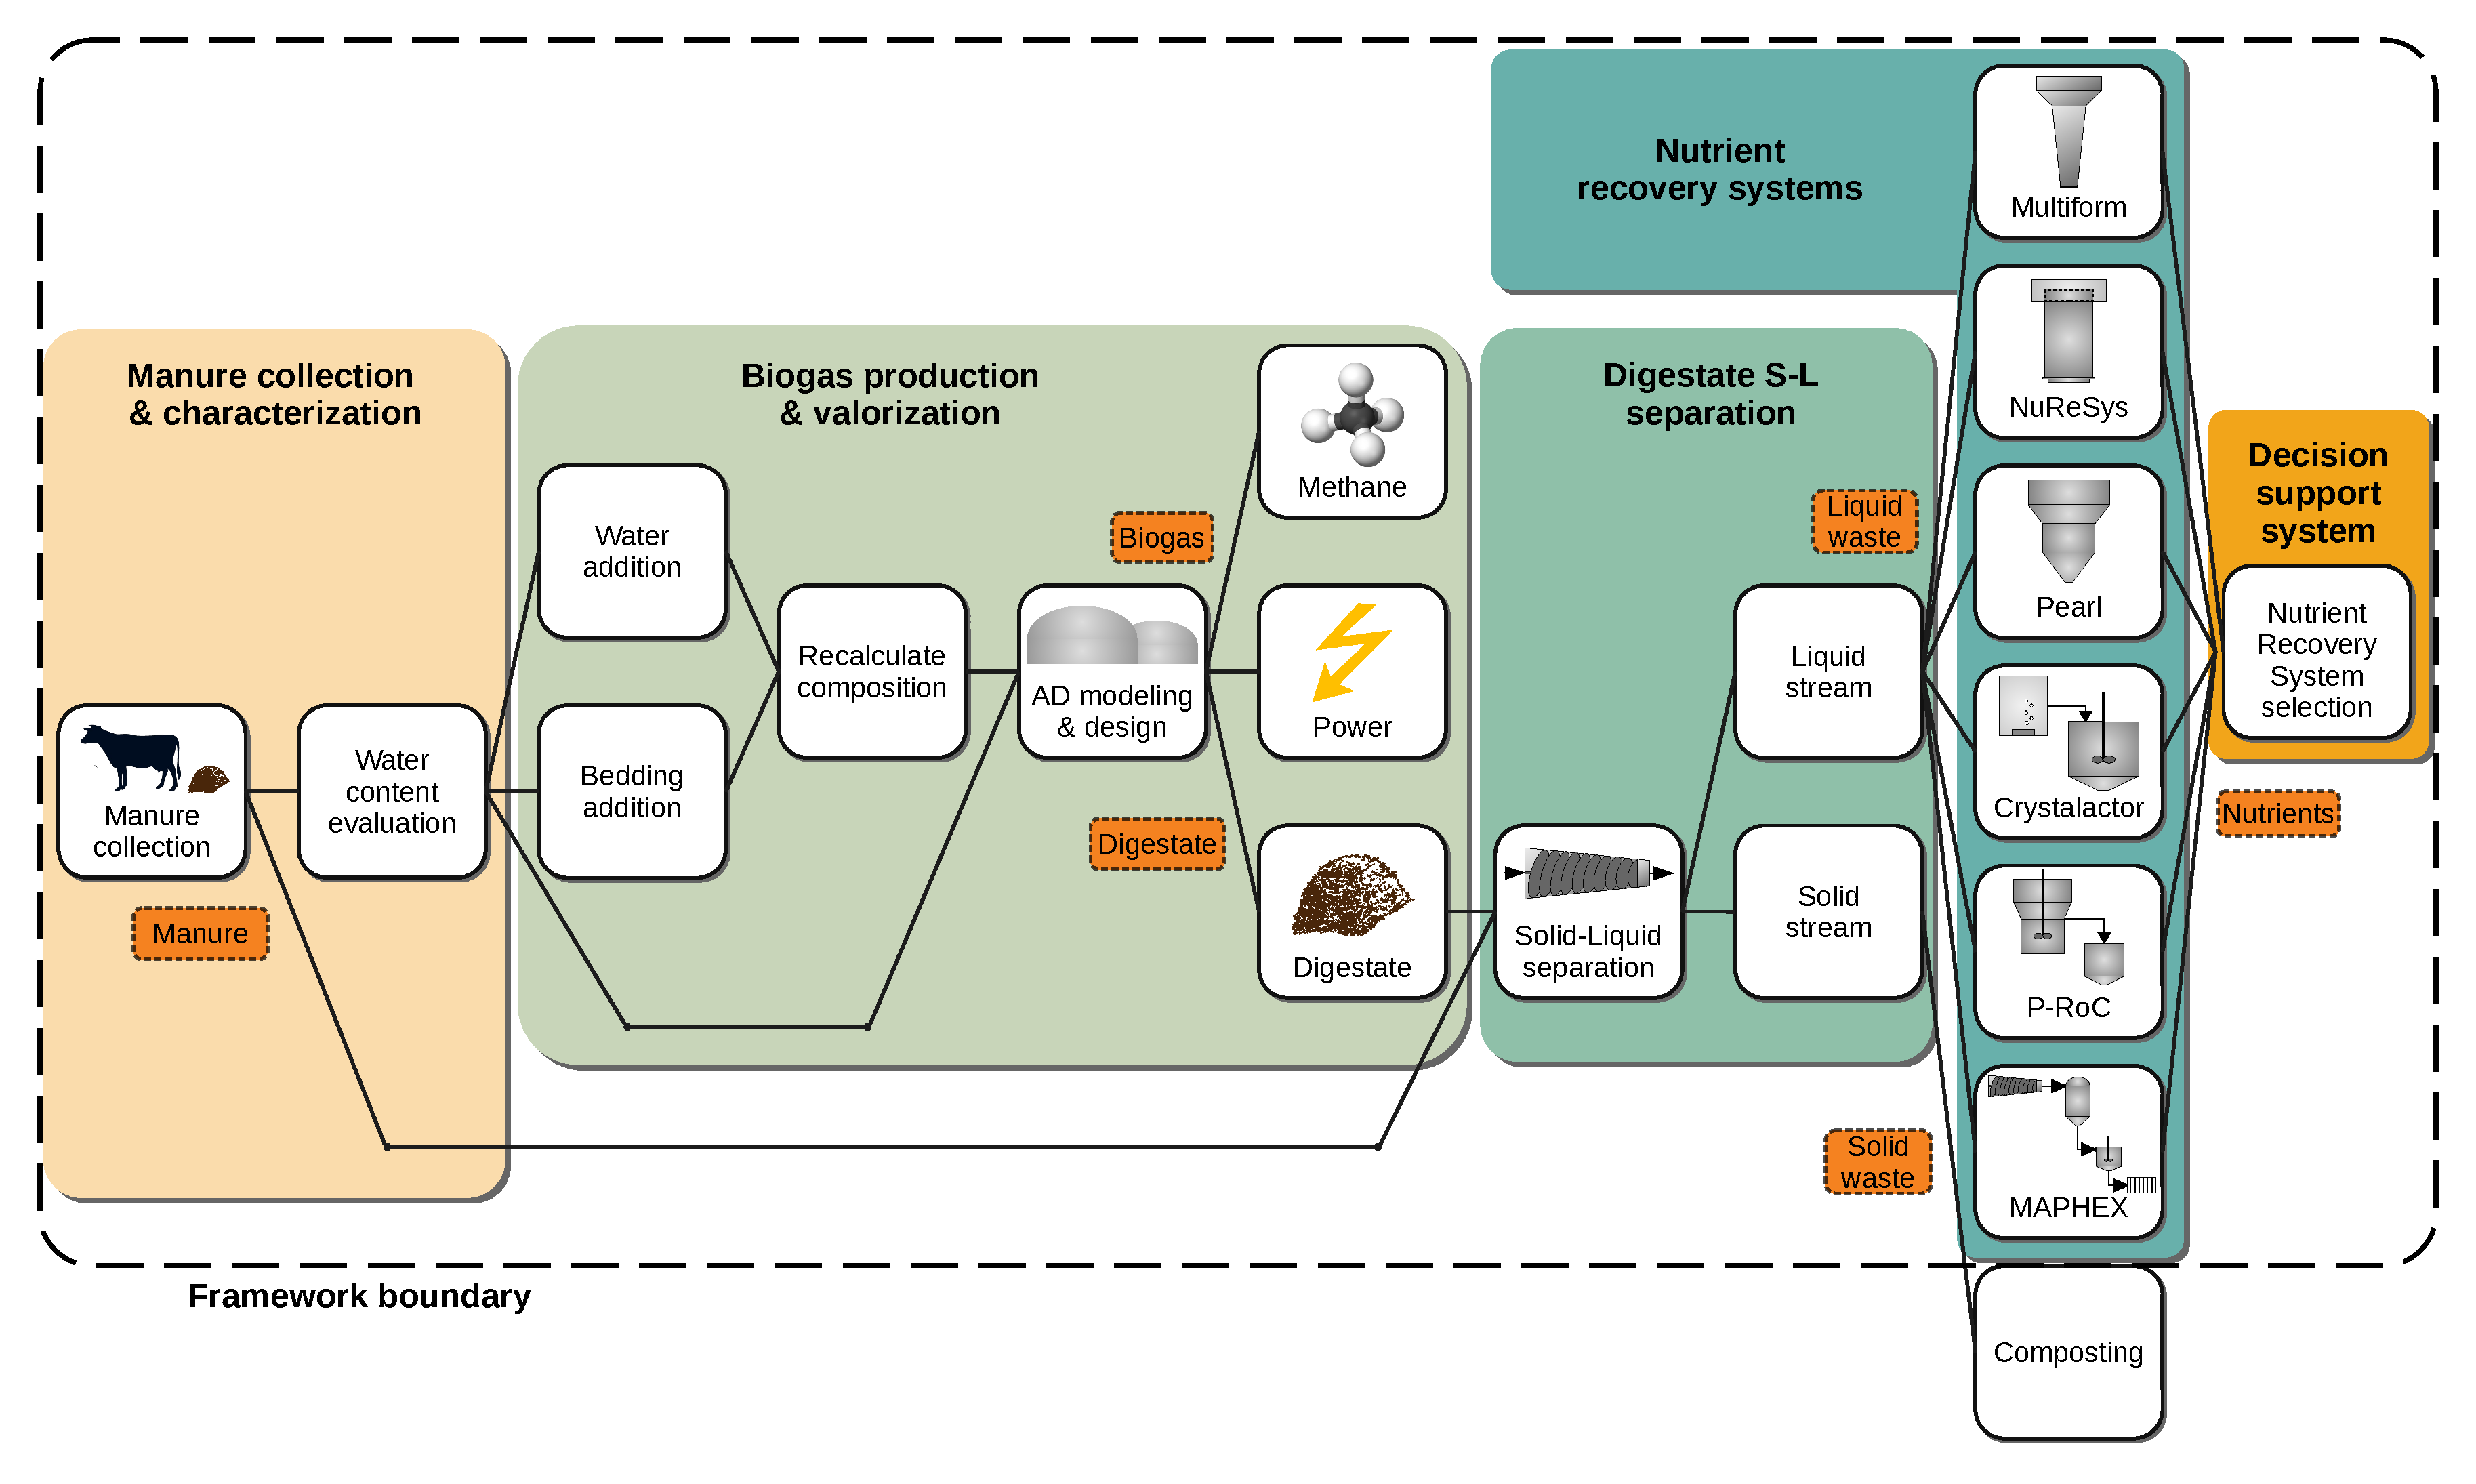
\includegraphics[width=\linewidth, trim=1cm 1cm 1cm 1cm, clip]{gfx/Chapter4/Process_Flowsheet2.pdf} 
	\caption{Process flowsheet for manure management and phosphorus recovery stages included in COW2NUTRIENT.}
	\label{fig:flowsheet}
\end{figure}

\subsubsection{Manure conditioning}
It is considered that the collection of manure does not involve any cost, since CAFOs have manure collection systems already installed. All manure produced is assumed to be collected. If the anaerobic digestion (AD) stage is implemented, a preconditioning stage is considered to adjust the water content of the waste. US EPA determines that the content of total solids in manure should be less than 15\% \citep{AgSTARHandbook}, as shown in Figure 6S of the Supplementary Material. Therefore, additional water may be added to reduce the solids content in manure before the AD stage.

\subsubsection{Anaerobic digestion}
Anaerobic digestion is a microbiological process that breaks down organic matter in the absence of oxygen. It involves four stages, hydrolysis, acidogenesis, acetogenesis, and methanogenesis; producing a mixture of gases mainly composed of methane and carbon dioxide (biogas), and a decomposed organic substrate (digestate). The model of the anaerobic digester is formulated through the mass balances of the species involved in the production of biogas and digestate. A detailed description of the digester modeling can be found in \citet{Leon}. As a result of the AD process, a fraction of organic phosphorus and nitrogen are transformed in their inorganic forms. To evaluate the amount of organic nutrients transformed into inorganic phosphorus and nitrogen, data available in literature was considered, resulting in an increase of 24\% and 16\% over the original inorganic ammonia and phosphate respectively, as shown in Table 5S of the Supplementary Material. Correlations to estimate the capital cost and operating and management costs (O\&M) as a function of the animal population of CAFOs were developed using data from the US EPA AgSTAR program \citep{AgSTAR2003} and the USDA \citep{USDA_OM} respectively. We refer the reader to the Supplementary Material for further information.

\subsubsection{Biogas purification}
Before transforming biogas into marketable products, a purification stage has to be carried out to remove H\textsubscript{2}S, H\textsubscript{2}O, and NH\textsubscript{3}. The removal of H\textsubscript{2}S is performed in a bed of ferric oxide through the production of Fe\textsubscript{2}S\textsubscript{3} operating at a temperature range of 25-50\textdegree C. The bed regeneration is carried out using oxygen to produce elemental sulfur and ferric oxide (Fe\textsubscript{2}O\textsubscript{3}). Water and ammonia are adsorbed using a pressure swing adsorption system (PSA) with zeolite 5A as adsorbent material, operating at low temperature (25\textdegree C) and moderate pressure (4.5 bar). The assumed recovery for NH\textsubscript{3} and H\textsubscript{2}O is 100\%. For further details about the modeling of the biogas purification stage, we refer the reader to previous works \citep{Leon, MartinHernandez}.

\subsubsection{Biogas valorization}
Two final added value products have been considered, methane and electricity, since they can be obtained through relatively simple processes and there exists developed markets for them.

\paragraph{Methane production}
The process considered for methane production is the removal of CO\textsubscript{2} using a PSA system with a bed of zeolite 5A, since this process was demonstrated as the optimal biogas upgrading process by \citet{MartinHernandez2020}, where further details about the modeling of the PSA system can be found.

\paragraph{Electricity production}
Electricity is produced from biogas through a gas turbine. A Brayton cycle consisting of double-stage compression system, one for the air stream and one for the biogas stream, is considered. Polytropic compression is assumed, with a polytropic index of 1.4 and an efficiency of 85\% \citep{moran2010fundamentals}. The adiabatic combustion of methane contained in the biogas is assumed, with a pre-heating of the biogas-air mixture, considering the combustion chamber as an adiabatic furnace. An air excess of 20\% with respect to the stoichiometric needs, and 100\% conversion of the reaction are assumed. Further details for electricity production can be found in \citet{MartinHernandez}.

\subsubsection{Solid-liquid separation}
Nutrients contained in organic waste (manure or digestate, depending on whether AD is carried out or not) are present in both organic and inorganic forms. Organic nutrients are chemically bonded to carbon, and they have to be converted into their inorganic forms through a mineralization process to be available for the vegetation to grow. Organic nutrients are mainly contained in the solid phase of organic waste. Inorganic nutrients are water soluble, and they are mostly present in the liquid phase, or bounded to soluble minerals. They are immediately available to plants, including algae involved during the occurrence of HABs. To recover the inorganic fraction of nutrients, a solid-liquid separation stage is implemented, keeping the inorganic nutrients in the liquid stage, which will be further processed, and the organic nutrients in the solid phased, which can be composted to mineralize nitrogen and phosphorus and be further used as fertilizers. The study of organic waste composting is out of the scope of this work.

Based on the evaluation reported by \citet{MollerSLsep}, a screw press is the technology selected to carry out the solid-liquid separation stage since it is the most cost-efficient
equipment. The partition coefficients for the different components are shown in Table 6S of the Supplementary Material. Assuming the discretization of units due to the commercial sizes available, the investment and operating costs for the screw press equipment are presented in Figure 9S of the Supplementary Material.

\subsubsection{Phosphorus recovery}
The technologies to recover inorganic phosphorus can be classified in three categories: struvite-based phosphorus recovery, calcium precipitates-based phosphorus recovery, and physical separation systems. Table \ref{table:techs_description} shows the classification and characteristics of the evaluated technologies. Regarding struvite-based systems, the formation of struvite has been widely described in the  literature, mainly focused on phosphorus recovery from wastewater \citep{rahaman_modeling_2014, Battistoni}. 
%Experimental data available to evaluate the efficiency and feasibility of P recovery through struvite formation are usually developed for municipal wastewater. 
However, cattle organic waste shows some characteristics that hinder struvite formation, including high ionic strength, which reduces the effective concentration of ions; and the presence of calcium ions competing for phosphate ions \citep{Yan2016}, which inhibits a selective recovery by phosphorus precipitation. The high variability in the manure composition, as a function of the geographic area, the animal feed, etc., represents an additional challenge for nutrient recovery \citep{Tao}. Therefore, specific correlations for livestock waste to estimate the molar fraction of $\text{PO}_{4}^{3-}$ and $\text{Ca}^{2+}$ recovered as struvite as a function of the amount of calcium contained in the waste were developed in a previous work \citep{MartinStruvite}. 

Among the different products obtained by the different processes, only struvite generates income. Calcium precipitates lacks of a well-established market as fertilizer, and therefore no sales of this product are considered. MAPHEX produces an organic solid rich in nutrients, but with a lower nutrient density compared with struvite, hindering transportation of this product and decreasing its market value. Therefore, we have assumed that no income is obtained from this product. Nevertheless, the recovered products allow phosphorus distribution from CAFO releases to phosphorus-deficient areas.

All technologies considered are at or near commercial stage. We note that, for all the technologies evaluated, the installation of several P recovery units in parallel arrangement is considered if the amount of waste to be processed exceeds the treatment capacity of the system. The description of the processes, and the correlations used to estimate the struvite formed, equipment cost, and operating costs are collected in the Section 2.2.4 of the Supplementary Material.

\begin{sidewaystable}[]
	\centering
	\caption{Description of phosphorus recovery technologies systems by COW2NUTRIENT framework. $x_{Ca^{2+}:PO_{4}^{3-}}$ refers to the $\text{Ca}^{2+}/\text{PO}_{4}^{3-} \ \text{molar ratio}$. $n_i$ denotes the number of units of the technology $i$ installed.}
	\label{table:techs_description}
	% Please add the following required packages to your document preamble:
	% \US EPAckage{booktabs}
	\resizebox{\columnwidth}{!}{
		\begin{tabular}{@{}ccccccccc@{}}
			\toprule
			Technology   & Company                                                                       & Technology type                                                            & \begin{tabular}[c]{@{}c@{}}Technology\\ readiness level\end{tabular} & \begin{tabular}[c]{@{}c@{}}Phosphorus recovery\\ efficiency (\%)\end{tabular} & 
			\begin{tabular}[c]{@{}c@{}}Treatment capacity\\ $\left(\frac{\text{kg\textsubscript{P-PO4}}}{\text{day} \cdot \text{unit}}\right)$ \end{tabular} & \begin{tabular}[c]{@{}c@{}}CAPEX\\ $\left(\frac{\text{MM USD}}{\text{unit}}\right)$ \end{tabular} & \begin{tabular}[c]{@{}c@{}} OPEX\\ $\left(\frac{\text{USD}}{\text{\text{kg\textsubscript{P-PO4}}}}\right)$ \end{tabular} & Reference \\ \midrule
			Multiform    & Multiform Harvest                                                             & Struvite-based                                                             & 9                                                                    & $\frac{0.798 \cdot 100}{1+\left(x_{Ca^{2+}:PO_{4}^{3-}} \cdot 0.576\right)^{2.113}}$   &38.5       &       1.1 &   15.42 & 1  \\
			
			Crystalactor & \begin{tabular}[c]{@{}c@{}}Royal Haskoning\\ DHV\end{tabular}                 & Struvite-based                                                             & 9                                                                    & $\frac{0.798 \cdot 100}{1+\left(x_{Ca^{2+}:PO_{4}^{3-}} \cdot 0.576\right)^{2.113}}$     & 137.7           &    $2.3 + 0.71 \cdot n_{\text{Crystalactor}}$      &  2.12 & 2  \\
			
			NuReSys      & \begin{tabular}[c]{@{}c@{}}Nutrient Recovery\\ Systems\end{tabular}           & Struvite-based                
			& 9                                                                    & $\frac{0.798 \cdot 100}{1+\left(x_{Ca^{2+}:PO_{4}^{3-}} \cdot 0.576\right)^{2.113}}$   & 204.0          &     1.38   &   6.22 &  1 \\
			
			Pearl 500       & Ostara                                                                        & Struvite-based                                                             & 9                                                                    & $\frac{0.798 \cdot 100}{1+\left(x_{Ca^{2+}:PO_{4}^{3-}} \cdot 0.576\right)^{2.113}}$            &         65.0    &  2.3 &  7.54 & 3 \\
			
			Pearl 2K       & Ostara                                                                        & Struvite-based                                                             & 9                                                                    & $\frac{0.798 \cdot 100}{1+\left(x_{Ca^{2+}:PO_{4}^{3-}} \cdot 0.576\right)^{2.113}}$            &      250.0   &   3.1  & 7.54 & 1 \\
			
			Pearl 10K       & Ostara                                                                        & Struvite-based                                                             & 9                                                                    & $\frac{0.798 \cdot 100}{1+\left(x_{Ca^{2+}:PO_{4}^{3-}} \cdot 0.576\right)^{2.113}}$            &         1250.0    &  10.0 &  7.54 & 4 \\
			
			P-RoC        & \begin{tabular}[c]{@{}c@{}}Karlsruhe Institute\\ of Technology\end{tabular}   & \begin{tabular}[c]{@{}c@{}}Calcium \\ precipitates-based\end{tabular}      & 6                                                                    & 60                      & 24.3     &  \begin{tabular}[c]{@{}c@{}}Tailored design based\\on waste flow processed. \\ See Section 2.2.4.4 of \\ Supplementary Material.	\end{tabular}   &     23.22 - 167.8  & 5  \\
			
			MAPHEX       & \begin{tabular}[c]{@{}c@{}}University of Pennsylvania\\ and USDA\end{tabular} & \begin{tabular}[c]{@{}c@{}}Modular phases\\ separation system\end{tabular} & 7                                                                    & 90                                                      & 18.5   &   0.3    &    110.8  & 6, 7  \\ \bottomrule
	\end{tabular}}
	\begin{tablenotes}
		\scriptsize
		\item 1: \citet{Pearl2Kcost2}
		\item 2: \citet{egle_phosphorus_2016}
		\item 3: \citet{Pearl500cost1}
		\item 4: \citet{Pearl10Kcost1}
		\item 5: \citet{ehbrecht_p-recovery_2011}
		\item 6: \citet{church_novel_2016}
		\item 7: \citet{church_versatility_2018}
	\end{tablenotes}
\end{sidewaystable}

\subsubsection{Incentives for the installation of nutrient recovery systems}
COW2NUTRIENT can evaluate the effect of different kinds of incentives on the economic performance of the nutrient recovery systems. These incentives can be received as a result of the recovery of phosphorus, in the form of P-credits, or for the generation of electricity or biomethane, in form of Renewable Energy Certificates (REC) and Renewable Identification Numbers (RIN) respectively. Renewable Energy Credits are a mechanism implemented in the US which guarantees that energy is generated from renewable sources, providing a system for trading produced renewable electricity. Each produced renewable megawatt-hour generates one REC, that can be sold separately from the electricity commodity itself and can be used to meet regulatory requirements by generators, trades, or end-users. On the other hand, RINs are identification numbers assigned to batches of biofuel, allowing their tracking through the production, purchase, and final usage. The allocation of RINs is associated with the allocation of incentives for the generation bio-fuels. 
The considered values for the different incentives are listed in Table 4S of the Supplementary Material.

\subsection{Multi-criteria decision model}
The determination of the most suitable nutrient management process is not a trivial procedure since multiple criteria play a critical role at the decision-making stage. COW2NUTRIENT performs the selection of P recovery technologies considering information concerning environmental, economic, and technology readiness dimensions. The integration of these dimensions is justified by the need to find the most suitable system for each CAFO by balancing operating cost and efficiency in the mitigation of nutrient pollution according to the local environmental vulnerability to eutrophication. Finally, the technical maturity of each system is also considered to assess the development level of the different processes. Therefore, a multi-criteria decision analysis (MCDA) model was developed to address the selection of the most suitable phosphorus recovery systems for each studied CAFO. The workflow of the MCDA model is summarized in Figure \ref{fig:MCDA_SMAA}.

\begin{figure}[h]
	\centering
	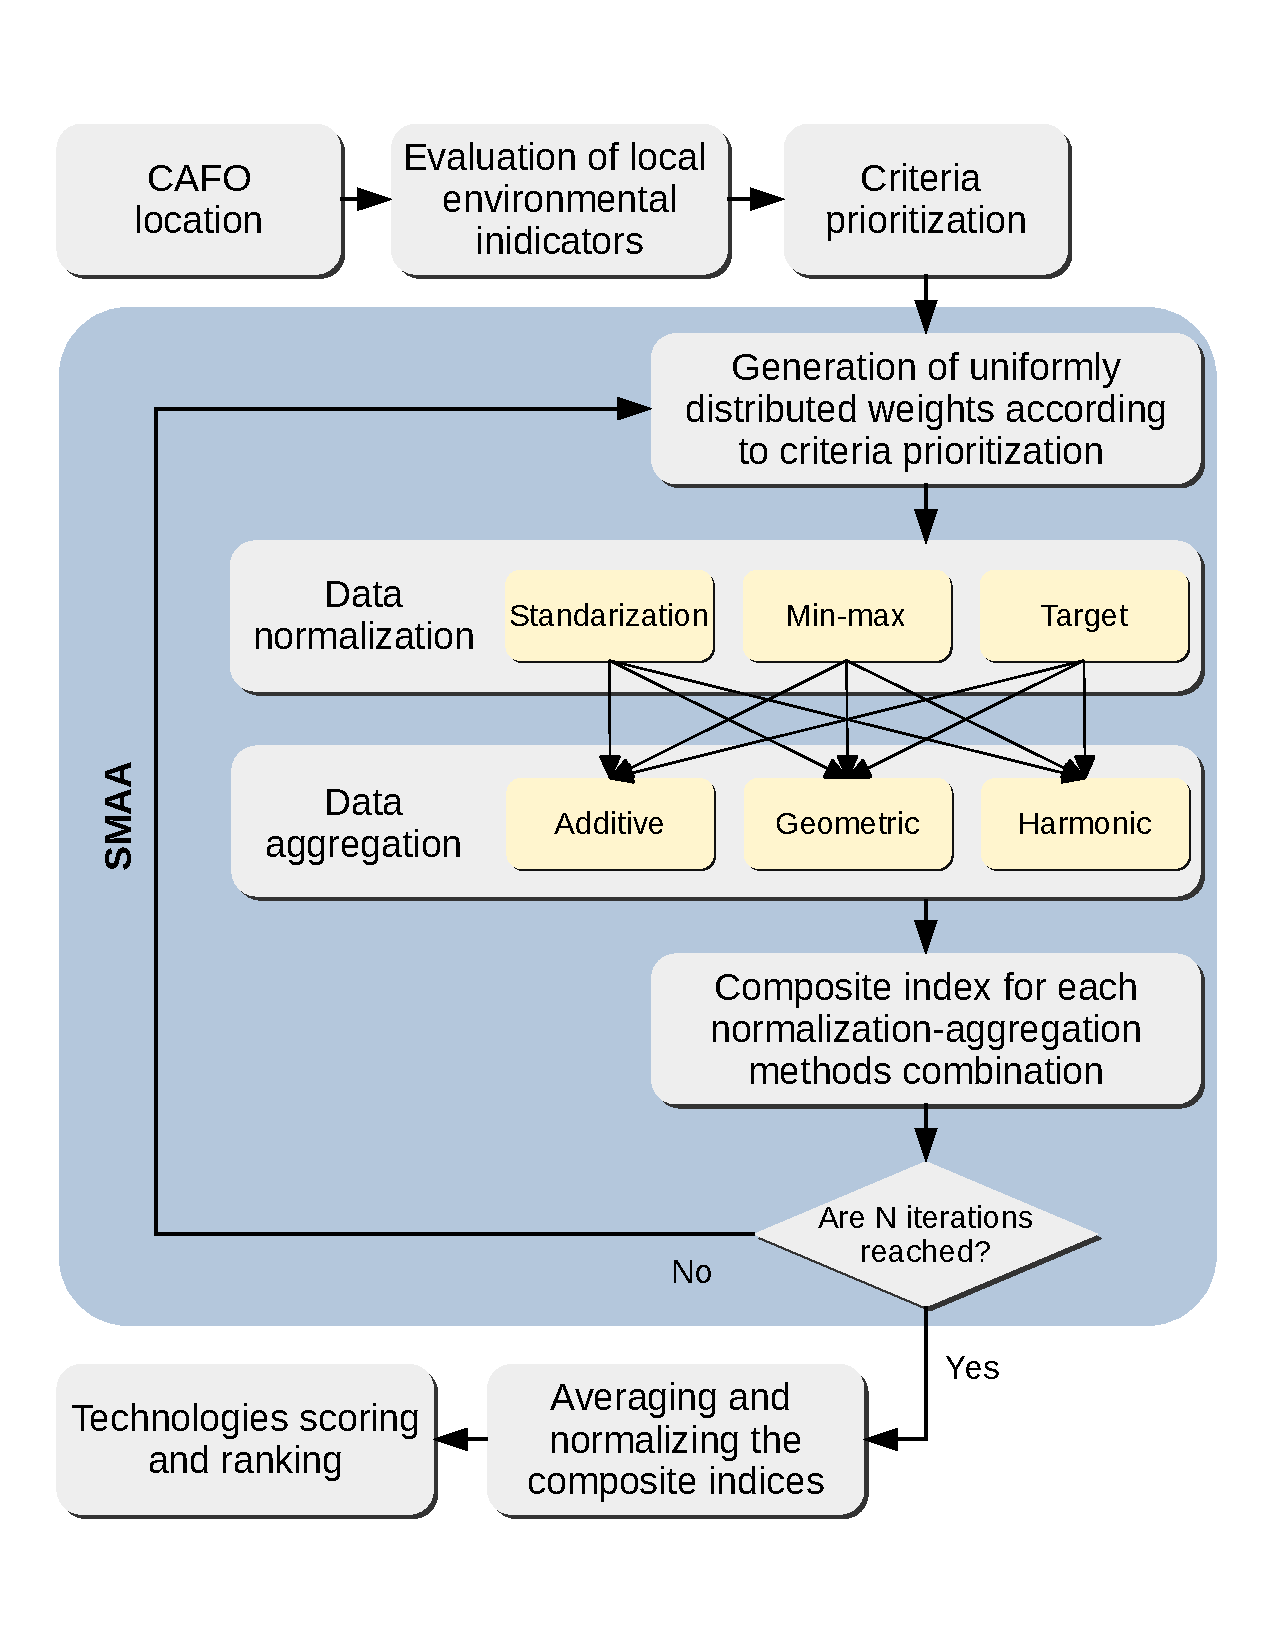
\includegraphics[width=0.9\linewidth, trim={0cm 1cm 0cm 1cm},clip]{gfx/Chapter4/MCDA_SMAA.pdf} 
	\caption{Flowsheet for the MCDA model.}
	\label{fig:MCDA_SMAA}
\end{figure}

Five criteria are combined in a composite index for the assessment of the environmental, economic, and technology maturity dimensions of the different technologies. Two environmental criteria are studied to assess the performance of the different technologies to mitigate phosphorus releases from CAFOs, i.e., the fraction of phosphorus recovered, and the potential environmental threat for the local ecosystem of the effluents containing the non-recovered phosphorus evaluated through the eutrophication potential of the effluents. The economic aspect is considered by means of two criteria, the economic barrier for the implementation of P recovery processes, measured in terms of capital cost, and the overall economic performance of the systems, which is evaluated through the net present value (NPV) \citep{sinnott2014chemical}. Finally, the technological maturity of the different technologies is considered though the technology readiness level (TRL) index. The construction of a composite index integrating these criteria is composed of three steps: criteria normalization, weighting, and aggregation \citep{MarcoCinelli2020}.

\subsubsection{Data normalization}
Since each criteria has a different range of potential values, they must be normalized to a common scale to allow each criteria to be compared with the others. However, the composite index can be affected by the normalization technique used. In order to study the robustness of the composite index obtained, and to address the uncertainty originated by data normalization, normalized data using standardization, min-max, and target normalization methods is calculated \citep{HandbookCompositeIndicators}.

\begin{table}[p]
	\centering
	\caption{Criteria preference as a function of the GIS-based environmental indicators for nutrient pollution.} \label{table:criteria_preference}
	\resizebox{\columnwidth}{!}{
	\begin{threeparttable}
		\begin{tabular}{@{}ccc@{}}
			\toprule
			\begin{tabular}[c]{@{}c@{}}Local environmental \\ indicators values\end{tabular}                                                                                              & Criteria ranking                                                                                                                                          & Description                                                                                                                                                                    \\ \midrule \\
			\begin{tabular}[c]{@{}c@{}}Condition 1:\\ TES $>$ TSI and \\ TES $>$ Soil fertility\\ \\ Condition 2:\\ TES = Unbalanced\end{tabular}                        & \begin{tabular}[c]{@{}c@{}}TRL $>$ NPV $>$ \\ Capital cost $>$ TP recovered $>$ \\ Eutrophication potential\end{tabular}  & \begin{tabular}[c]{@{}c@{}}Unbalanced phosphorus releases \\ but no immediate threat to \\ soil and water bodies. \\ \\ Prevalence of economic criteria for \\ nutrient recovery system selection.\end{tabular} \\ \\ \midrule \\
			\begin{tabular}[c]{@{}c@{}}Condition 1:\\ TSI $\geq$ TES or\\ TSI $\geq$ Soil fertility\\ \\ Condition 2:\\ TSI = Eutrophic or\\ Hypereutrophic\end{tabular}    & \begin{tabular}[c]{@{}c@{}}TRL $>$ \\ Eutrophication potential $>$ NPV $>$ \\ TP recovered $>$ Capital cost\end{tabular} & \begin{tabular}[c]{@{}c@{}}High Trophic State Index. \\ \\ Inmmediate environmental risk \\ due to potential algal blooms. \\ \\ Prevalence of environmental criteria \\ for nutrient recovery system selection.\end{tabular}    \\  \\ \\ \midrule \\
			\begin{tabular}[c]{@{}c@{}}Condition 1:\\ Soil fertility $\geq$ TES and \\ Soil fertility $>$ TSI \\ \\ Condition 2:\\ Soil fertility = Excessive\end{tabular} & \begin{tabular}[c]{@{}c@{}}TRL $>$ TP recovered $>$ \\ NPV $>$ Eutrophication potential $>$ \\ Capital cost\end{tabular}  & \begin{tabular}[c]{@{}c@{}}Excessive P in soil. \\ \\ Inmmediate environmental risk \\ due to potential P runoff. \\ \\ Prevalence of environmental criteria \\ for nutrient recovery system selection.\end{tabular}           \\    \\ \\ \midrule \\
			\multicolumn{1}{l}{\begin{tabular}[c]{@{}c@{}}Condition:\\ TES $\neq$ Saturated\\ and \\ TSI $\neq$ Eutrophic or\\ Hypereutrophic\\ and\\ Soil fertility $\neq$ Excessive\end{tabular}}      & \begin{tabular}[c]{@{}c@{}}TRL $>$ NPV $>$ \\ Capital cost $>$ TP recovered $>$ \\ Eutrophication potential\end{tabular}  & \multicolumn{1}{c}{\begin{tabular}[c]{@{}c@{}}No environmental risk.\\ \\ Prevalence of economic criteria for\\ nutrient recovery system selection.\end{tabular}}                                                     \\  \\ \bottomrule
		\end{tabular}
		\begin{tablenotes}
			\item TRL: Technology Readiness Level
			\item TSI: Trophic State Index
			\item TES: Techno-Ecological Synergy sustainability metric
			\item NPV: Net Present Value
			\item TP: Total Phosphorus
		\end{tablenotes}
	\end{threeparttable}
	}
\end{table}

\subsubsection{Criteria weighting}
The normalized criteria are weighted to set the relative importance of each criterion, prioritizing some criteria over others. This is needed in order to obtain a flexible decision method able to balance the operating cost of the systems and the P recovery efficiency as a function of the environmental vulnerability to eutrophication of each region. The minimization of the operating costs is prioritized in regions with low eutrophication risk, while the efficiency of P recovery is more relevant in regions affected by nutrient pollution. Therefore, the criteria are dynamically weighted according to the values of TSI, TES and Mehlich 3 phosphorus concentration in each region studied. The preference of criteria as a function of the environmental vulnerability to eutrophication is shown in Table \ref{table:criteria_preference}. On the one hand, if there is immediate environmental risk by nutrient pollution (i.e., high values for TSI or soil fertility), phosphorus recovery efficiency is prioritized over economic performance. Conversely, if there is environmental risk in the long run due to the unbalance between anthropogenic phosphorus releases and uptakes (negative value of TES indicator), or there is no potential environmental risk, the economic performance is prioritized over the phosphorus recovery efficiency. 
Finally, since the objective of this framework is to select P recovery systems that are feasible to install and operate in CAFOs, the TRL index is set as the criteria with highest preference in all cases in order to minimize the risk of selecting non-full-scale processes. As a result, the selection of processes with low TRL will be hampered unless they have good economic or environmental performance.

The procedure described above sets the prioritization of criteria, i.e., they can be sorted in order of importance. However, it does not provide an specific value for the weights, which values are unknown. In order to avoid the risk of biasing the decision-making procedure setting arbitrary values for the weights, a stochastic multi-criteria acceptability analysis (SMAA) is used to explore the weights space \citep{tervonen_implementing_2007}. Through this approach, the feasible space of each weight (i.e., the space delimited by the previous and the subsequent weights) is explored through the Monte Carlo method, retrieving a set of weights for all criteria according to the assigned order. The SMAA is formulated by defining the set of $n$ weights ($\omega$) as a non-negative set which elements must sum 1, as shown in Eqs. \ref{eq:weight_def_1} and \ref{eq:weight_def_2}.

\begin{align}
& \omega_{j} \geq 0 \ \forall \ j \ \in \ {n} \label{eq:weight_def_1}\\
& \sum_{j=1}^{n} \omega_{j} = 1  \label{eq:weight_def_2} \\
%\end{align}
%
%\begin{align}
& \omega_{j1} \geq \omega_{j2} \geq ... \geq \omega_{jn} \label{eq:weight_def_3}
\end{align}

The preference information of the criteria, defined through the ranking of the criteria shown in Table \ref{table:criteria_preference}, is expressed as a sequence of inequality constraints, Eq. \ref{eq:weight_def_3}. A detailed description of the SMAA method can be found in \citet{tervonen_implementing_2007}. A number of Monte-Carlo simulations $\left(N\right)$ of 100 is assumed as a trade-off between computational cost and MCDA model performance.

\subsubsection{Criteria aggregation}
The aggregation stage merges the weighted criteria, resulting in the composite index. 
Similarly to the normalization stage, different aggregation methods are evaluated to improve the robustness of the solutions retrieved by the framework. Different aggregation schemes denote different degrees of compensability between indicators, i.e. a deficit in one criteria can be fully, partially, or not compensated by a surplus in other criteria \citep{MarcoCinelli2020}. Three aggregation functions are evaluated including full compensation (additive aggregation) and partial compensation schemes (geometric and harmonic aggregation methods). Nine composite indexes are obtained for each P recovery technology combining normalization and aggregation techniques, as shown in Figure \ref{fig:MCDA_SMAA}.
Finally, the composites indexes are normalized in a range from 0 to 1 and ranked to determine the most suitable P recovery process for the CAFO under study.

\subsection{Framework limitations}
The main limitations of the proposed framework lie in the uncertainty of the input data. On the one hand, since the data regarding the animal number, type of animals, and location of CAFOs are reported by the state environmental protection agencies of each state, they are considered reliable. On the other hand, to estimate the local vulnerability to phosphorus pollution throughout the contiguous US, HUC8 spatial resolution has been chosen as a trade-off solution between spatial accuracy and data uncertainty. However, more accurate results can be obtained if reliable data for phosphorus level in soils, fertilizer  application rates, etc. are available for higher spatial resolution. Particularly, further studies for developing more accurate correlations to estimate the fraction of phosphorus available to plants based on soil type and climate conditions in each region would improve the accuracy of the assessment of local risk to phosphorus pollution. Additionally, since the proposed framework is focused on phosphorus recovery for freshwater nutrient pollution prevention and control, the recovery of other resources contained in livestock manure (such as organic carbon and nitrogen) is not considered in this study.

\subsection{Case study}
\subsubsection{Study region}
The Great Lakes area, located in North America, is selected in order to demonstrate the implementation of nutrient management systems at CAFOs using the COW2NUTRIENT framework. This region is selected because its high concentration of CAFO facilities, resulting in significant nutrient releases that contribute to frequent HABs and eutrophication episodes,
as well as to the nutrient legacy accumulated over time \citep{sayers2019satellite, han2012historical}. The evaluation and implementation of phosphorus recovery systems at CAFOs already in operation at the US states of Pennsylvania \citep{Pennsylvania_CAFOS}, Ohio \citep{Ohio_CAFOS}, Indiana \citep{Indiana_CAFOS}, Michigan \citep{Michigan_CAFOS}, Wisconsin \citep{Wisconsin_CAFOS}, and Minnesota \citep{Minnesota_CAFOS} are performed using the criteria prioritization based on the GIS indicators describing 
the environmental impact of nutrient pollution shown
in Table \ref{table:criteria_preference}. The states of Illinois and New York, and the Canadian province of Ontario, which are also part of the Great Lakes area, are not included due to the unavailability of reliable information about their CAFOs. A description of the studied states listing the animal units, annual manure generation, and annual phosphorus releases by the year 2019, disaggregated for dairy and beef cattle, is collected in Table 10S of the Supplementary Material. 

It should be noted that, accordingly to the US regulatory definition of CAFOs, only intensive livestock facilities with 300 animal units or more are considered in this study \citep{CAFO_definition}, resulting in the evaluation of 2,217 CAFOs. An animal unit is defined as an animal equivalent of 1,000 pounds (453.6 kg) live weight \citep{animal_unit_definition}. Animal units is used as a unit to measure the size of CAFOs due to the presence of different types of animals in the CAFOs, i.e. beef or dairy cows, and animals of different age, including heifers, calves, and adult animals. Different types of animals result in different manure generation rates and composition. Therefore, the different types of animals within each studied CAFO are normalized using the definition of animal units to estimate the amount and composition of the manure generated.

\subsubsection{Scenarios description}
Two scenarios have been evaluated, the deployment of only phosphorus recovery systems, and the integration of these processes with AD and electricity production processes. 
Incentives for the recovery of phosphorus based on the work of \citet{sampat_economic_2018} are considered, assuming a phosphorus credit value of 22 USD/kg\textsubscript{P recovered} for both scenarios. We note that this value is significantly lower than the economic impact of P release from livestock waste, valued in 74.5 USD/kg\textsubscript{P released} \citep{sampat2021valuing}. Additionally, in the scenario considering the production biogas-based electricity, a value of Renewable Energy Certificates (fixed electricity selling price) of 60 USD per MWh generated is assumed. Finally, a discount rate of 7\% is considered in both scenarios. 

\section{Results}
\subsection{Implementation of phosphorus recovery systems in the Great Lakes area}
Table \ref{table:techs_intalled} summarizes the results of the phosphorus recovery process selection in the Great Lakes area.
It can be observed that only three out of the six commercial processes evaluated are selected to be installed. All selected processes recover P in the form of struvite, which is a valued product that can be sold, generating income. Although the Ostara Pearl process also produces struvite, it results in larger operating costs than the technologies selected. Conversely, P-RoC recovers phosphorus in the form of calcium-based precipitates. This product lacks a well-established market, and therefore it does not generate income. In addition, P-RoC is the technology with the lowest TRL, which hampers the selection of this process. The selection of modular phosphorus recovery systems, such as MAPHEX, which due to economies of scale are especially suitable for small livestock facilities, is largely prevented by the absence of small-scale CAFOs. Therefore, a sub-set of three technologies is obtained. Therefore, it can be concluded that the selection of this pool of three technologies amongst the six systems evaluated is mainly driven by economic factors. Additionally, the low TRL of P-RoC also hampers the selection of this process.

The selection of the most suitable technology for each studied CAFO among the sub-set comprised by Multiform, Nuresys, and Crystalactor systems is based on the CAFO scale and local eutrophication risk, as it is discussed in the following sections.

\begin{table}[h]
	\centering
	\caption{Distribution and characteristics studied CAFOs, and phosphorus recovery processes selected. Only selected technologies are included in the table.} \label{table:techs_intalled}
	\resizebox{\columnwidth}{!}{
		\begin{threeparttable}
			\begin{tabular}{@{}ccccccccccc@{}}
				\toprule
				\multirow{3}{*}{State} & \multirow{3}{*}{\begin{tabular}[c]{@{}c@{}}CAFO\\ average size\\ (animal units)\end{tabular}} & \multirow{3}{*}{\begin{tabular}[c]{@{}c@{}}Number\\ of \\ CAFOs\end{tabular}} & \multirow{3}{*}{\begin{tabular}[c]{@{}c@{}}Manure \\ generated \\ (ton/year)\end{tabular}} & \multirow{3}{*}{\begin{tabular}[c]{@{}c@{}}P \\ recovered \\ (ton/year, (\%))\end{tabular}} & \multicolumn{6}{c}{\begin{tabular}[c]{@{}c@{}}Number of phosphorus\\ recovery systems installed\end{tabular}} \\ \cmidrule(l){6-11} 
				&                                                                                                &   &                                                                         &                                                                                       & \multicolumn{2}{c}{Multiform}       & \multicolumn{2}{c}{NuReSys}       & \multicolumn{2}{c}{Crystalactor}  \\ \cmidrule(lr){6-7} \cmidrule(lr){8-9} \cmidrule(lr){10-11}
				&                                                                                                &            &                                                                &                                                                                       & S1               & S2               & S1              & S2              & S1              & S2              \\ \midrule
				Indiana           & 1,574.41                                                                                        & 119                                                                         & $2.48 \cdot 10^6$ & 1558.8 (78.7)                            & 116               & 113               & 0               & 0               & 3               & 6               \\
				Michigan          & 2,461.52                                                                                        & 144                                                                        & $4.76 \cdot 10^6$ & 3004.4 (79.0)                                                                               & 127              & 113               & 16              & 30              & 1               & 1               \\
				Minnesota         & 634.23                                                                                        & 1,487                                                                         & $1.13 \cdot 10^7$ & 6938.1 (76.9)                                                                                & 1,477                & 1,476                & 0               & 0               & 10              & 11              \\
				Ohio              & 2,415.24                                                                                        & 53                                                                         & $1.68 \cdot 10^6$ & 1055.8   (78.6)                                                                              & 50               & 47               & 1               & 3               & 2               & 3               \\
				Pennsylvania      & 1,495.94                                                                                        & 131                                                                         & $2.59 \cdot 10^6$ & 1633.2  (78.9)                                                                              & 124               & 119               & 6               & 11              & 1               & 1               \\
				Wisconsin         & 2,628.19                                                                                        & 283                                                                        & $1.02 \cdot 10^7$ & 6510.5 (79.4)                                                                               & 262              & 255              & 6               & 7              & 15              & 21              \\ \bottomrule
		\end{tabular}
		\begin{tablenotes}
			\item S1: Phosphorus recovery systems only.
			\item S2: Phosphorus recovery systems coupled with AD and electricity production.
		\end{tablenotes}
	\end{threeparttable}
	}
\end{table}

\subsubsection{Effect of CAFOs scale on selecting P recovery systems}
A relationship between CAFOs size and the selected technologies can be observed in Table \ref{table:techs_intalled}. This relationship is also observed in Figures \ref{fig:PTechs_Distribution} and \ref{fig:Capital_TechSelected}. Multiform is the predominant phosphorus recovery process. Furthermore, we observe that in those states with smaller CAFOs (Minnesota and Indiana) the selection of Multiform is more predominant than in states with larger CAFOs. On the contrary, in the states with large CAFOs or with outliers representing large facilities, (such as Ohio and Wisconsin) Crystalactor is selected for some facilities.
Additionally, NuReSys is a technology also selected for medium-size CAFOs.

The integration of biogas production and upgrading affects the selection of P recovery processes as a consequence of the high investment expenditures associated to the installation of AD processes. These large costs blur the capital investment differences between different P recovery processes. As a result, the MDCA model promotes the implementation of technologies with better long-term economic performance (lower operating costs), such as NuReSys and Crystalactor, in spite of the fact that they involve larger investments costs than other technologies like Multiform, as shown in Figure \ref{fig:PTechs_Distribution_AD}. 

\begin{figure}[h!]
	\centering
	\begin{subfigure}[t]{0.7\linewidth}
		\centering
		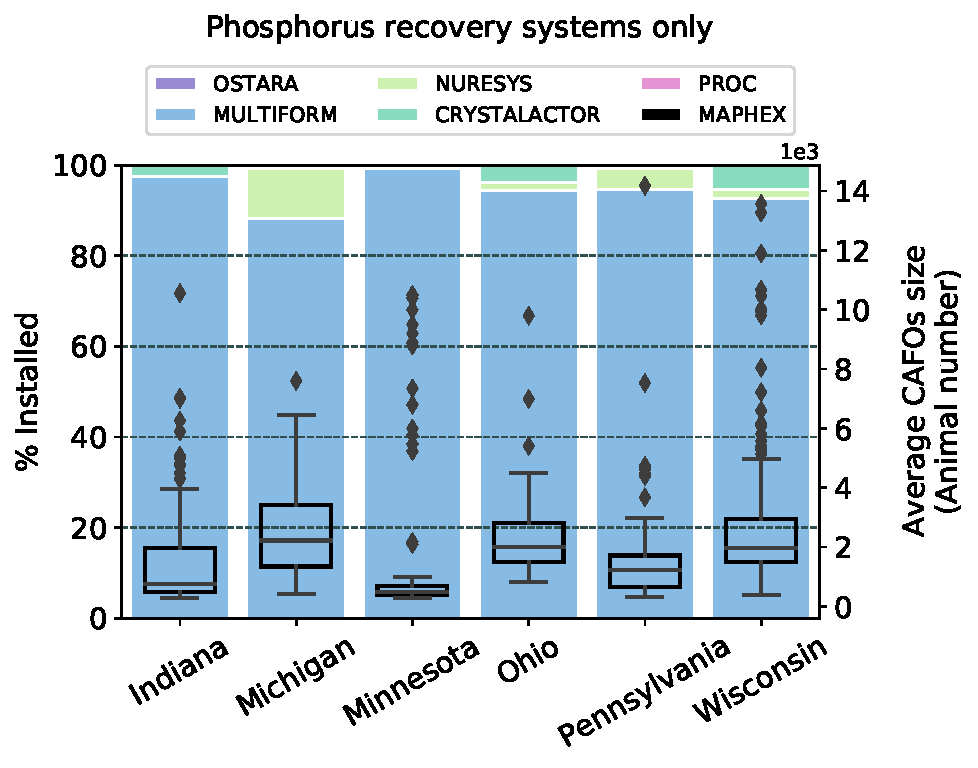
\includegraphics[width=\linewidth]{gfx/Chapter4/TechsDistribution_Pcredits22_REC0.pdf} 
		\caption{Phosphorus recovery systems only.}
		\label{fig:PTechs_Distribution_NoAD}
	\end{subfigure}
%	\hspace{0.5em}
	\begin{subfigure}[t]{0.7\linewidth}
		\centering
		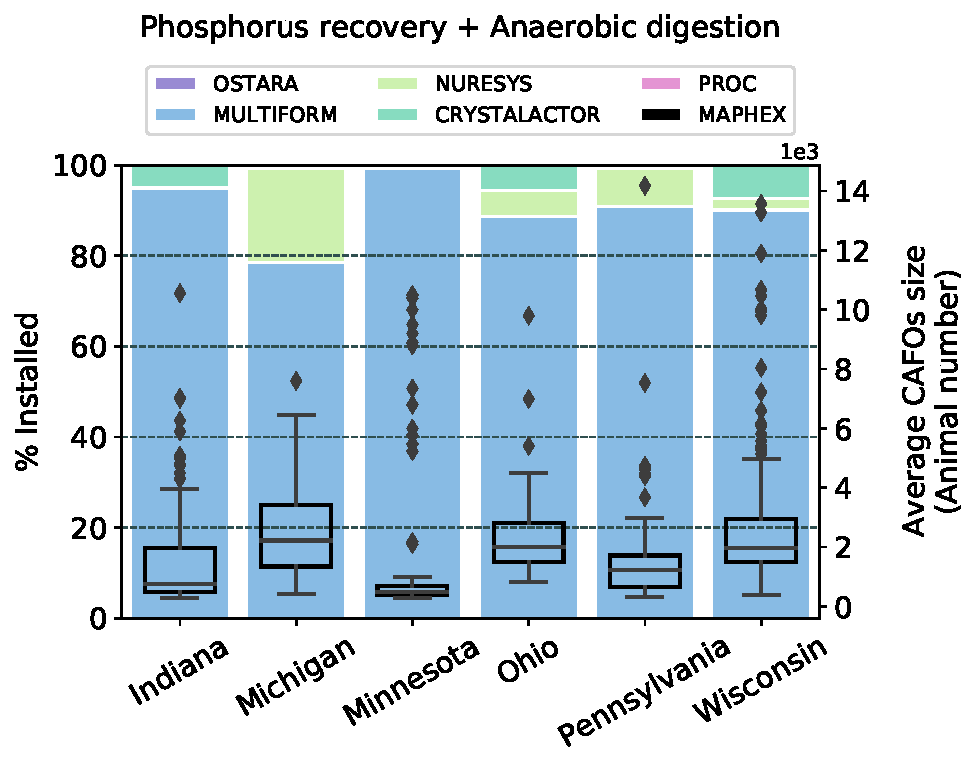
\includegraphics[width=\linewidth]{gfx/Chapter4/TechsDistribution_Pcredits22_REC60.pdf}
		\caption{Phosphorus recovery systems coupled with AD and electricity production.}
		\label{fig:PTechs_Distribution_AD}
	\end{subfigure}
	
	\caption{Distribution of the phosphorus recovery systems selected for the CAFOs in the Great Lakes area. The boxplots represent the distribution of CAFO sizes in each studied state.}
	\label{fig:PTechs_Distribution}
\end{figure}

Based on the data illustrated in Figures \ref{fig:Capital_TechSelected} to \ref{fig:NetRev_TechSelected}, a preliminary screening of P recovery systems can be performed based on the size of the CAFOs. If the installation of only nutrient recovery systems is considered, Multiform can be selected for CAFOs with sizes up to 5,000 animal units, NuReSys can be selected for CAFOs with a size between 2,000 and 5,000 animal units, and Crystalactor is selected for CAFOs larger than 5,000 animal units. For the scenario integrating anaerobic digestion and phosphorus recovery processes, Multiform is mostly selected for CAFOs up to 4,000 animal units, although it is also selected in some larger CAFOs, NuReSys are mostly selected for CAFOs between 2,000 and 6,000 animal units, while the size range for the selection of Crystalactor is similar to the previous case. The operating costs are shown in Figure \ref{fig:OPEX_TechSelected}. It can be observed that the operating cost of Multiform is larger than NuReSys, and in turn the operating cost of this one is larger than Crystalactor, showing an opposite pattern than capital costs.

\subsubsection{Effect of local eutrophication risk on the selection of P recovery systems}
The results obtained reveal that CAFOs scale is the main driver for the selection of phosphorus recovery technologies. However, the role of the environmental vulnerability to eutrophication can be appreciated in those CAFOs where two different systems show similar economic performance. From the results illustrated in Figure \ref{fig:NetRev_TechSelected}, it can be observed that Multiform and NuReSys technologies are selected for CAFOs with similar size. However, the economic performance of the second technology is better as consequence of the lower operating expenses and larger net revenues of this technology. Although both technologies have similar phosphorus recovery yield, Multiform shows better environmental performance since the eutrophication potential of its output streams is lower than NuReSys effluents. This difference in eutrophication potential between both technologies is mainly driven by the higher nitrogen recovery of Multiform. Therefore, in those locations that are highly vulnerable to nutrient pollution, the solution proposed by the COW2NUTRIENT framework is driven more by environmental criteria than by economic criteria, resulting in the selection of the Multiform process.

\begin{table}[h]
	\centering
	\caption{Economic results per state for installing phosphorus recovery systems in the studied states of the Great Lakes area.} \label{table:economic_results}
	\resizebox{0.9\columnwidth}{!}{
		\begin{threeparttable}
			\begin{tabular}{@{}ccccccc@{}}
				\toprule
				\multirow{2}{*}{State} & \multicolumn{2}{c}{\begin{tabular}[c]{@{}c@{}}CAPEX\\ (MM USD)\end{tabular}} & \multicolumn{2}{c}{\begin{tabular}[c]{@{}c@{}}OPEX\\ (MM USD/year)\end{tabular}} & \multicolumn{2}{c}{\begin{tabular}[c]{@{}c@{}}Net revenue\\ (MM USD/year)\end{tabular}} \\ \cmidrule(lr){2-3} \cmidrule(lr){4-5} \cmidrule(lr){6-7} 
				& S1                                          & S2                                          & S1                                           & S2                                           & S1                                                             & S2                                                             \\ \midrule
				Indiana                & 145.58                                       & 325.00                                      & 21.18                                        & 34.16                                        & 19.32                                                          & 11.88                                                          \\
				Michigan               & 191.09                                      & 480.19                                      & 36.74                                       & 55.92                                        & 41.00                                                          & 32.15                                                          \\
				Minnesota              & 1,591.40                                       & 2,866.31                                      & 140.74                                         & 251.58                                        & 39.61                                                           & -46.15                                                          \\
				Ohio                   & 68.30                                       & 179.29                                      & 12.95                                         & 20.32                                        & 14.46                                                          & 10.80                                                          \\
				Pennsylvania           & 148.16                                       & 332.03                                      & 21.46                                        & 35.03                                       & 20.82                                                          & 12.95                                                          \\
				Wisconsin              & 396.24                                      & 1,009.47                                      & 73.55                                        & 117.80                                        & 95.44                                                          & 74.14                                                         \\ \bottomrule
			\end{tabular}
			%	}
			\begin{tablenotes}
				\item S1: Phosphorus recovery systems only.
				\item S2: Phosphorus recovery systems coupled with AD and electricity production.
			\end{tablenotes}
		\end{threeparttable}
	}
\end{table}

\subsection{Economic results}
The capital expenditures (CAPEX), operating expenses (OPEX), and net revenues (difference between incomes and operating expenses) associated with the deployment of the nutrient management systems are listed per state in Table \ref{table:economic_results}. For the scenario considering the installation of only phosphorus recovery processes, the CAPEX and OPEX are 2,540.77 MM USD and 185.65 MM USD per year respectively. If the integration of biogas production and upgrading to power with phosphorus management is considered, the CAPEX and OPEX increase up to 5,192.29 MM USD and 267.51 MM USD per year respectively. It can be observed that, due to the high CAPEX of biogas production and upgrading stages, the net revenues decrease from 230.65 MM USD per year for the scenario considering only phosphorus recovery systems to 95.77 MM USD per year if the processes for phosphorus recovery and AD are combined.

\begin{figure}[h!]
	\centering
	\begin{subfigure}[t]{0.7\linewidth}
		\centering
		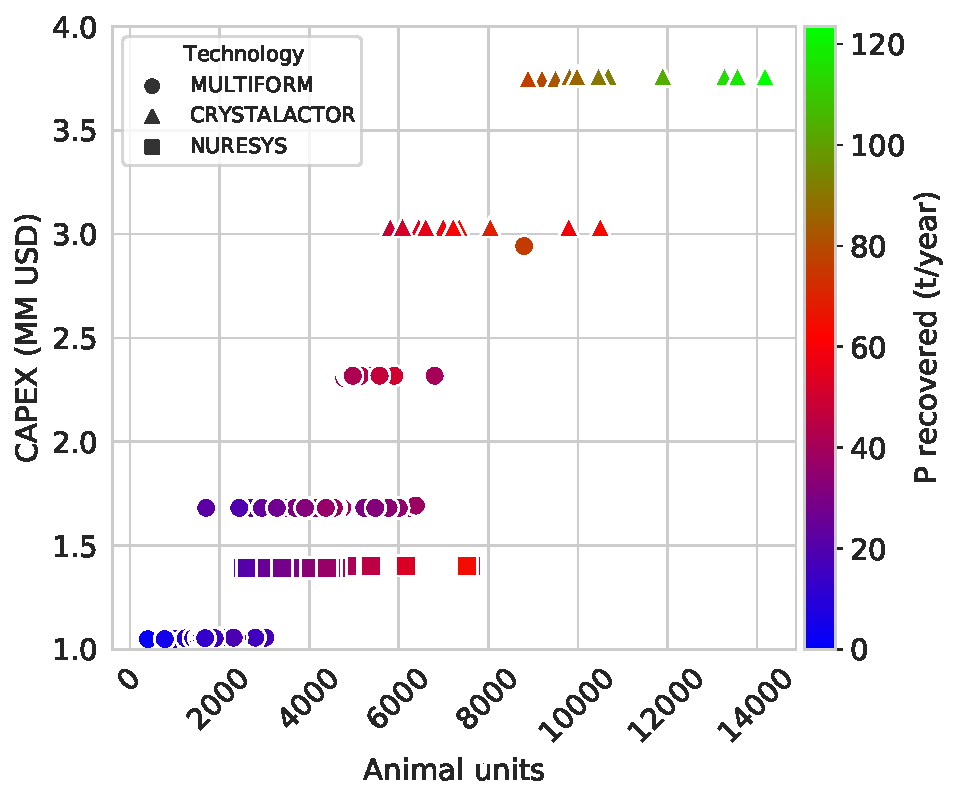
\includegraphics[width=\linewidth]{gfx/Chapter4/Capital_TechSelected_Pcredits22_REC0.pdf} 
		\caption{Phosphorus recovery systems only.}
		\label{fig:Capital_TechSelected_Pcredits22_REC0}
	\end{subfigure}
	
	\begin{subfigure}[t]{0.7\linewidth}
		\centering
		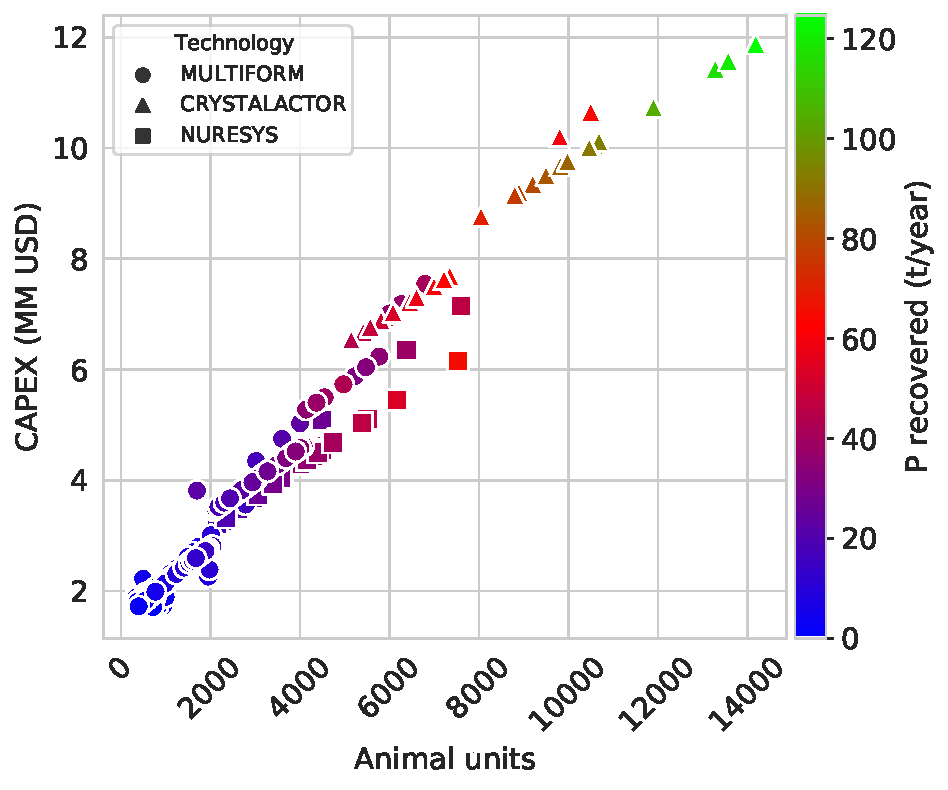
\includegraphics[width=\linewidth]{gfx/Chapter4/Capital_TechSelected_Pcredits22_REC60.pdf}
		\caption{Phosphorus recovery systems coupled with AD and electricity production.}
		\label{fig:Capital_TechSelected_Pcredits22_REC60}
	\end{subfigure}
	
	\caption{Capital expenses for deploying phosphorus recovery systems in the studied CAFOs. The dots represent the P recovery technologies installed in the studied CAFOs.}
	\label{fig:Capital_TechSelected}
\end{figure}


\begin{figure}[h!]
	\centering
	\begin{subfigure}[t]{0.7\linewidth}
		\centering
		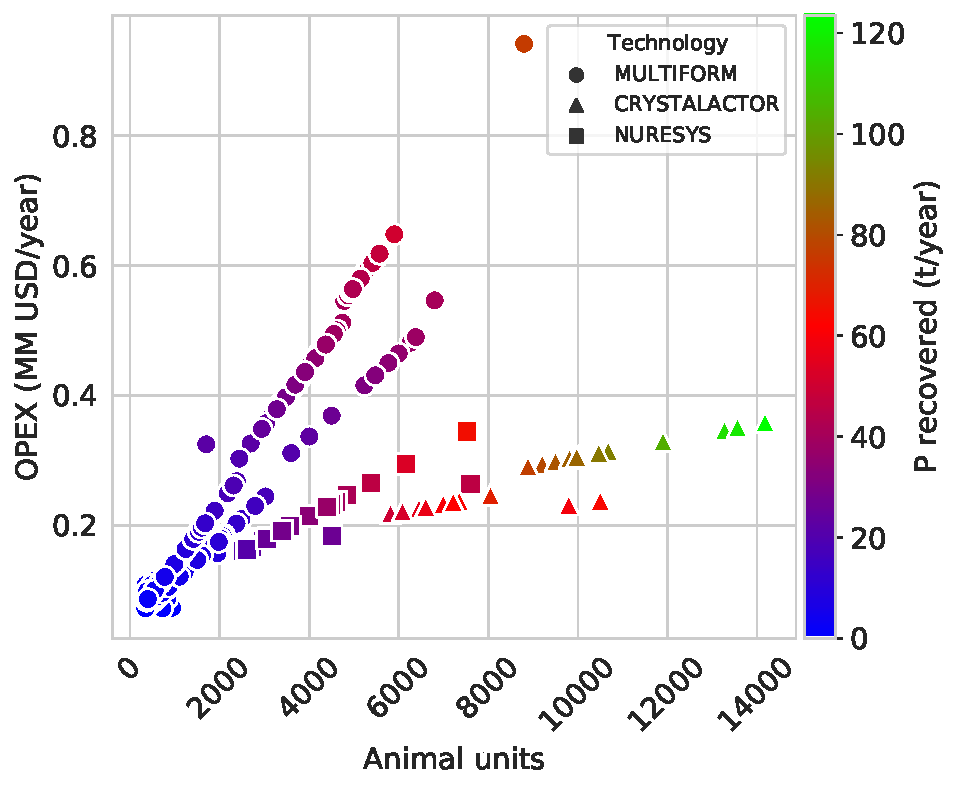
\includegraphics[width=\linewidth]{gfx/Chapter4/Amortized_TechSelected_Pcredits22_REC0.pdf} 
		\caption{Phosphorus recovery systems only.}
		\label{fig:OPEX_TechSelected_Pcredits22_REC0}
	\end{subfigure}
	
	\begin{subfigure}[t]{0.7\linewidth}
		\centering
		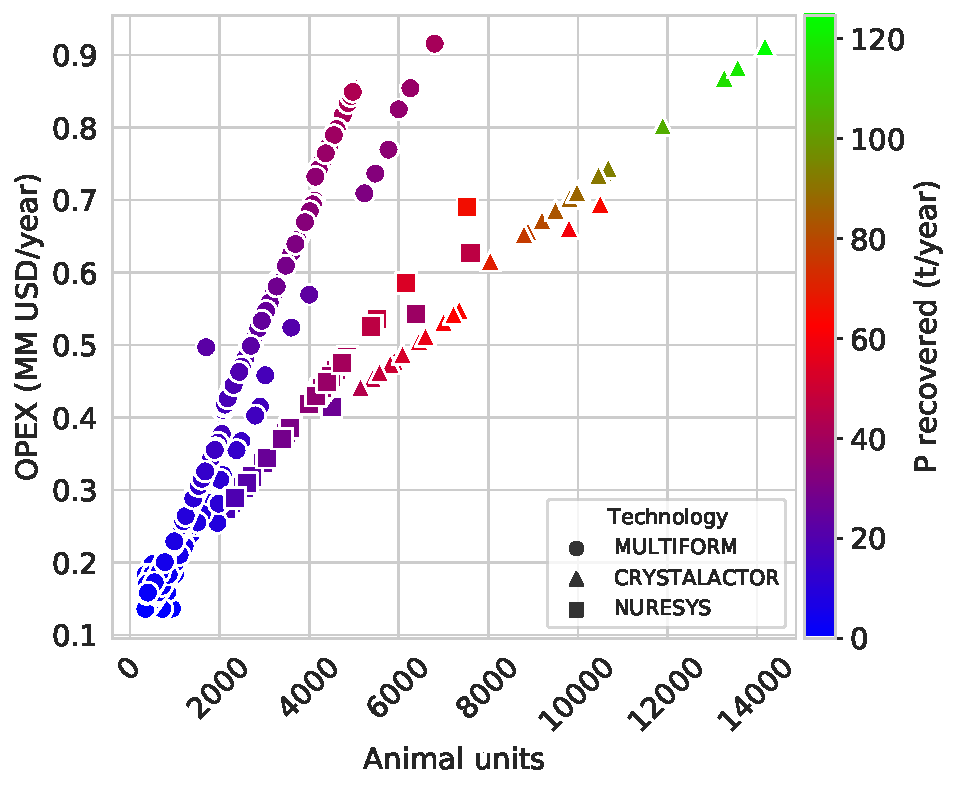
\includegraphics[width=\linewidth]{gfx/Chapter4/Amortized_TechSelected_Pcredits22_REC60.pdf}
		\caption{Phosphorus recovery systems coupled with AD and electricity production.}
		\label{fig:OPEX_TechSelected_Pcredits22_REC60}
	\end{subfigure}
	
	\caption{Operating expenses for deploying phosphorus recovery processes in the studied CAFOs. The dots represent the P recovery technologies installed in the studied CAFOs.}
	\label{fig:OPEX_TechSelected}
\end{figure}

Figures \ref{fig:Capital_TechSelected} and \ref{fig:OPEX_TechSelected} show the evolution of CAPEX and OPEX of the P recovery technologies installed at the livestock facilities studied as a function of CAFOs scale. Figure \ref{fig:Capital_TechSelected_Pcredits22_REC0} shows the CAPEX when the implementation of only P recovery systems is considered. We observe that CAFOs are grouped in sets selecting the same P recovery technology. This is because the manufacturers standardize the size of each P recovery technology, which in turn determines the maximum waste processing capacity of each technology (as shown in Table \ref{table:techs_description}). This results in the use of the same P recovery equipment, and thus the same CAPEX, for all the CAFOs generating waste below the maximum processing capacity. Likewise, we note different CAPEX values for the implementation of the same P recovery technology. This is a consequence of installing of multiple in-parallel P recovery units to increase the processing capacity of such technology, since the waste generated in that CAFO exceeds its maximum processing capacity. It can also be appreciated that CAFOs with similar size might result in the installation of different technologies, or a different number of units of the same technology.
This is because, although CAFOs can have a similar number of animal units, the type of the animals can be different, resulting in the generation of different amounts of manure. 
In the case of considering biogas production and upgrading, illustrated in Figure \ref{fig:Capital_TechSelected_Pcredits22_REC60}, the required CAPEX increases significantly, blurring the differences in the capital investment between different P recovery processes observed in Figure \ref{fig:Capital_TechSelected_Pcredits22_REC0} into the cost of the whole system. The integration of AD and electricity production also results in the increase of the OPEX, as shown in Figure \ref{fig:OPEX_TechSelected}.

\begin{figure}[h!]
	\centering
	\begin{subfigure}[t]{0.7\linewidth}
		\centering
		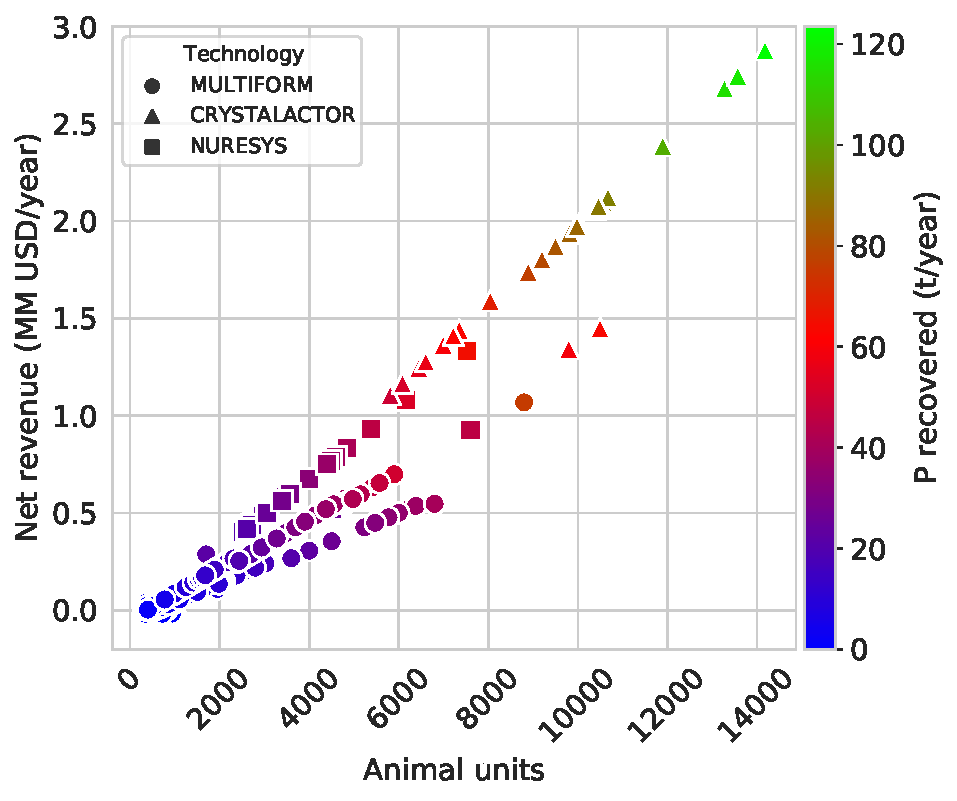
\includegraphics[width=\linewidth]{gfx/Chapter4/NetRev_TechSelected_Pcredits22_REC0.pdf} 
		\caption{Phosphorus recovery systems only.}
		\label{fig:NetRev_TechSelected_Pcredits22_REC0}
	\end{subfigure}
	
	\begin{subfigure}[t]{0.7\linewidth}
		\centering
		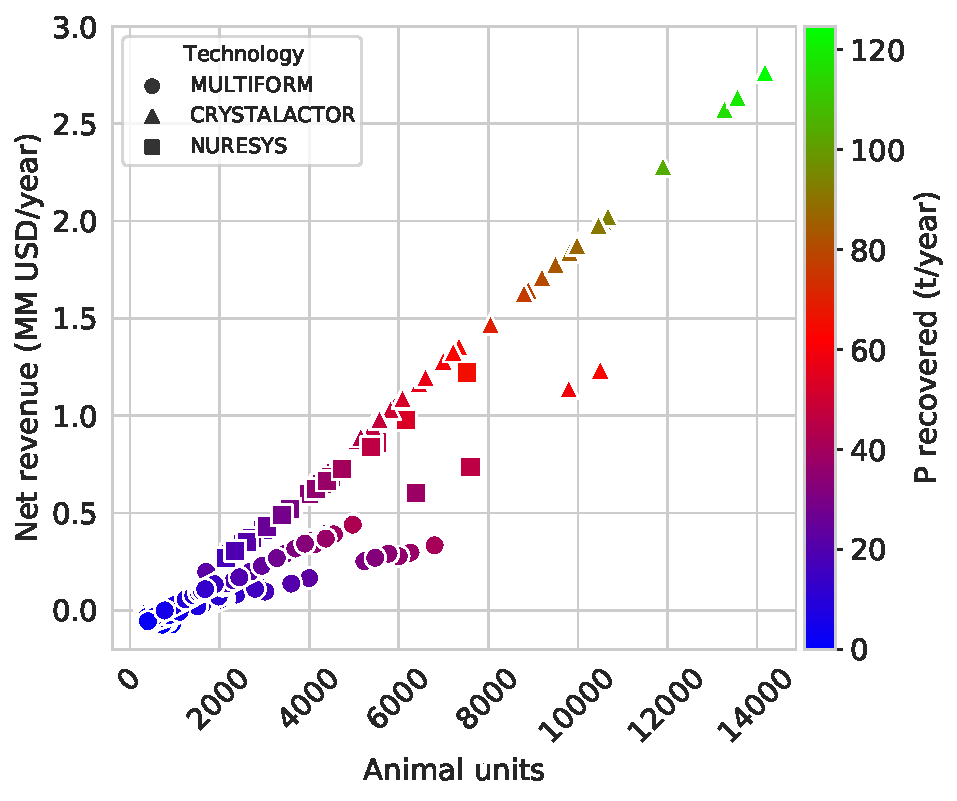
\includegraphics[width=\linewidth]{gfx/Chapter4/NetRev_TechSelected_Pcredits22_REC60.pdf}
		\caption{Phosphorus recovery systems coupled with anaerobic digestion and electricity production.}
		\label{fig:NetRev_TechSelected_Pcredits22_REC60}
	\end{subfigure}
	
	\caption{Net revenue from the phosphorus recovery processes selected in the studied CAFOs. The dots represent the P recovery technologies installed in the studied CAFOs.}
	\label{fig:NetRev_TechSelected}
\end{figure}

The net revenue of the installed nutrient management systems according with the economic parameters described at the beginning of the section is shown in Figure \ref{fig:NetRev_TechSelected}. We observe a pattern characterized by the increase of the net revenues with the increase of CAFOs size. However, the implementation of P recovery technologies in CAFOs below 1,000 animal units, and below 2,000 animal units if biogas production and upgrading is also considered, result in economic looses. Additionally, the integration of these processes slightly decreases the net revenues of the systems installed for phosphorus recovery.


\section{Discussion}
\subsection{Economic implications}
In this work, fixed incentives for P recovery and biogas-based electricity generation have been considered as starting point to explore the effect of the application of incentives in the implementation of P recovery technologies, either standalone or integrated with biogas production and upgrading processes.		
The results shown in Figure \ref{fig:NetRev_TechSelected} reveal the effect of the economies of scale in the net revenues from the implementation of P recovery technologies in the Great Lakes area are highly dependent on the economies of scale, i.e., the larger the amount of waste to be treated, the larger the net revenues obtained. However, while for the largest CAFOs significant profits are obtained, negative revenues (i.e., economic looses) are obtained for the smallest CAFOs, even for large P credits prices such as 22 USD/kg\textsubscript{P recovered}. This suggests that the implementation of fixed incentives is not a fair policy, since the small CAFOs are not profitable while they increase the profits of the largest CAFOs. Therefore, alternative incentive policies must be explored. \citet{sampat2019coordinated} studied the development of a coordinated management system for the treatment of cattle manure and P recovery. That framework captures the geographical phosphorus imbalance by proposing different prices for manure treatment that capture the regional remediation cost caused by P releases. They found that economic drivers are needed for a cost-effective recovery and redistribution of phosphorus, considering fixed incentives for P recovery up to 50 USD/kg\textsubscript{P} for this purpose. Therefore, further research about the effect of implementing dynamic incentives for P recovery is needed. These incentive policies can follow different schemes, such as progressive incentives for P recovery based on the amount of manure treated, or cooperative schemes where the profits from P recovery obtained by the largest livestock facilities are redistributed to the smallest CAFOs. This is a concept that has been studied for minimizing the costs of meeting greenhouse gases emission targets \citep{galan2018time}, and could be adopted for the reduction of P releases.

Furthermore, consideration should be given to the fair allocation of incentives in those scenarios where the available incentives budget is not enough to avoid economic looses in all CAFOs. In this regard, the fairness measure considered for budget allocation must be carefully selected among the existing schemes \citep{sampat2019fairness}. 
%As a result, we note that the following three factors should be considered in the design of incentive schemes: avoiding economic looses in all CAFOs, a fair distribution of the available incentives, and minimizing the cost of the incentives required in order to reduce the social impact of P recovery while mitigating environmental impacts.}}

\subsection{Phosphorus use efficiency}
Currently, manure or digestate in liquid phase is usually supplied as nutrient supplementation in croplands, or it is treated in either aerobic or anaerobic ponds. Solid phase processing is based on composting or drying. However, the high density of manure and digestate and low concentration of nutrient prevent an efficient redistribution of the phosphorus released from CAFOs to phosphorus-deficient areas \citep{burns2002phosphorus}. Therefore, the implementation of phosphorus recovery processes 
is a desirable measure for sustainable phosphorus management. We find that implementing struvite production processes considering incentives for P recovery of 22 USD/kg\textsubscript{P recovered} is economically feasible for CAFOs larger than 1,000 animal units if standalone P recovery technologies are implemented, and for CAFOs larger than 2,000 animal units if they are integrated with biogas production and upgrading processes. The requirement of large incentives to produce profit in most of the P recovery systems installed at CAFOs might raise the debate of whether it is worthwhile to implement P recovery systems; or if the economic resources should be allocated to simpler phosphorus management alternatives, such as the redistribution of either raw or pond-stored manure. In this regard, \citet{sampat2019coordinated} studied the separation of manure in liquid and solid phases, and their further transport to demanding allocations, considering a coordinated management system in Upper Yahara watershed (Wisconsin, United States). In addition, that study considered the implementation of economic incentives from 0 to 50 USD/kg\textsubscript{P}. However, the results showed that manure redistribution is not an economically viable technique for phosphorus recycling in this range of incentives. The main drawback of manure redistribution is the large transportation cost of both liquid and solid raw manure because of the high volume of these materials and their low phosphorus concentration. Therefore, the results reveal that on-site manure processing to generate valuable products (struvite) is more beneficial than manure redistribution.

The replacement of phosphorus from synthetic fertilizers by the recovered P, mitigating the dependency on fertilizers from non-renewable resources (phosphate rock), is an interesting alternative towards the sustainability of the agri-food sector. However, phosphorus availability for plants depends on several factors, including the P product used as fertilizer and soil pH level. Since struvite is the product recovered in all studied CAFOs, we will focus the discussion on this product.
\citet{vaneeckhaute2015efficiency} compared the bio-availability of several bio-based fertilizers, including struvite, to synthetic triple super phosphate (TSP). This study shows that P available in soil (measured as Prhizon) was a 45\% higher than TSP in acidic soils (pH=5.0), but 60\% lower in slightly basic soils (pH=7.9). Based on these data, one kilogram of manure processed for P recovery by struvite production can replace from $1.53\cdot 10^{-3}$ to $3.71\cdot 10^{-3}$ kg of TSP ($5.02 \cdot 10^{-3}$ kg of struvite are recovered per kilogram of manure processed). However, it must be noted that currently the cost of recovered P from manure (2.12-15.42 USD/kg\textsubscript{P recovered}, see Table \ref{table:techs_description}) is considerable larger than the cost of phosphorus from synthetic TSP (1.23  USD/kg\textsubscript{P}) \citep{fertilizers_price}. As a result, from an economic perspective the complete substitution of phosphate rock is currently hindered by the large recovery costs, in addition to a limited availability of resources recovered from waste, and henceforth further exploration on resource recovery from different wastes is required to achieve P circularity reducing the recovery costs, and increasing the amount of phosphorus from organic waste, including but not limited to livestock manure.

\section{Conclusion}
We presented a framework for the techno-economic evaluation and selection of phosphorus recovery systems considering the local vulnerability to phosphorus pollution through a GIS environmental model. A multi-criteria decision analysis model is used for the comparison and section of phosphorus recovery systems based on the economic performance and technological readiness level of the processes, and the eutrophication risk of the watershed where the studied CAFOs are located. Technologies for P recovery in the form of struvite are selected in all CAFOs studied. The selection of P recovery technologies is mainly driven by economic criteria, and the effect of the economies of scale is very significant. However, environmental criteria (P recovery efficiency, eutrophication potential of process effluents) are the decision criteria at some CAFOs where different technologies show similar economic performances. The results show that a preliminary screening of P recovery systems can be performed based on the size of CAFOs. Multiform can be selected for CAFOs with sizes up to 5,000 animal units,
NuReSys can be selected for CAFOs with a size between 2,000 and 5,000 animal units, and Crystalactor is selected for CAFOs larger than 5,000 animal units. The implementation of these systems in the Great Lakes area involves capital expenditures of 2.5 billion USD and operating costs of 186 million USD per year if only phosphorus recovery technologies are installed, and 5.2 billion USD and 268 million USD per year respectively if biogas production and upgrading are also considered. The implementation of fixed incentives of 22 USD/kg\textsubscript{P recovered} is considered to avoid economic looses due to P recovery costs impact in the economy of CAFOs. However, we find that that the implementation of
fixed incentives is not a fair policy, since the small CAFOs are not profitable while they increase the
profits of the largest CAFOs. The phosphorus recovered in the form of struvite from one kilogram of manure processed can replace from $1.53\cdot 10^{-3}$ to $3.71\cdot 10^{-3}$ kg of synthetic triple super phosphate, but incurring in significantly larger production costs (2.12-15.42 USD/kg\textsubscript{P recovered}) than synthetic fertilizer (1.23  USD/kg\textsubscript{P}). 

As part of future work, customized incentive policies adapted to the particularities of each livestock facility can be proposed in order to optimize the allocation of limited monetary resources. Additionally, it would be interesting to analyze the potential of crop-livestock integration as an alternative for phosphorus recycling to the implementation of physicochemical P recovery processes. Another interesting research line is the integration of multiple processes in order to recover additional valuable products from organic waste (such as biochar), adapting the concept of refinery to resource recovery from organic waste.

\section*{Acknowledgments} \label{section:Acknowledgments}
\addcontentsline{toc}{section}{Acknowledgments}
This research was supported in part by an appointment for E. Mart\'{i}n-Hern\'{a}ndez to the Research Participation Program for the Office of Research and Development, US EPA, administered by the Oak Ridge Institute for Science and Education through Interagency Agreement No. DW-89-92433001 between the US Department of Energy and the US Environmental Protection Agency. PSEM3 research group acknowledge funding from the Junta de Castilla y Le\'{o}n, Spain, under grant SA026G18 and grant EDU/556/2019.

\textbf{Disclaimer:} The views expressed in this article are those of the authors and do not necessarily reflect the views or policies of the US EPA. Mention of trade names, products, or services does not convey, and should not be interpreted as conveying, official US EPA approval, endorsement, or recommendation.

\section*{Bibliography}
\addcontentsline{toc}{section}{Bibliography}

\printbibliography[heading=none]
\end{refsection}
%\printbibliography[heading=none]